\documentclass{beamer}
\usepackage[UTF8,fontset=none]{ctex}
\usepackage{fontspec}
\usepackage{tikz}
\usetikzlibrary{arrows.meta,positioning,calc}
\usepackage{booktabs}
\usepackage{array}
\graphicspath{{assets/}}

\setCJKmainfont[
  Path=/System/Library/AssetsV2/com_apple_MobileAsset_Font7/54a2ad3dac6cac875ad675d7d273dc425010a877.asset/AssetData/,
  FontIndex=0,
  BoldFont=Kaiti.ttc,
  BoldFeatures={FontIndex=3}
]{Kaiti.ttc}
\setCJKsansfont[
  Path=/System/Library/AssetsV2/com_apple_MobileAsset_Font7/54a2ad3dac6cac875ad675d7d273dc425010a877.asset/AssetData/,
  FontIndex=0,
  BoldFont=Kaiti.ttc,
  BoldFeatures={FontIndex=3}
]{Kaiti.ttc}
\setCJKmonofont[Path=/Users/yrk/Library/Fonts/]{NotoSansCJKsc-Regular.otf}

\author[yrk队]{yrk队}
\title[问阶 AI 学习工作台]{问阶 AI 学习工作台}
\subtitle{多智能体个性化高校学习资源系统}
\institute[华中师范大学]{华中师范大学计算机学院}
\date{2026 年 7 月}
\usepackage{Tsinghua}

\definecolor{accentblue}{HTML}{2F80ED}
\definecolor{accentgreen}{HTML}{159D82}
\definecolor{accentorange}{HTML}{F2994A}
\definecolor{accentred}{HTML}{E85D75}
\setbeamertemplate{navigation symbols}{}
\setbeamertemplate{section in toc}[sections numbered]

\newcommand{\tagbox}[2]{\tikz[baseline=(x.base)]\node[fill=#1!12,draw=#1!28,rounded corners=2pt,inner xsep=5pt,inner ysep=2pt,text=#1,font=\scriptsize\bfseries](x){#2};}
\newcommand{\bigmetric}[3]{\begin{minipage}[t]{.29\linewidth}\centering{\color{#3}\fontsize{23}{25}\selectfont\bfseries #1}\par{\scriptsize #2}\end{minipage}}

\begin{document}
\begin{frame}
  \titlepage
\end{frame}

\begin{frame}{汇报提纲}
  \tableofcontents[sectionstyle=show,subsectionstyle=show/shaded/hide]
\end{frame}

\section{项目简介}

\begin{frame}{行业分析：政策与用户规模共同推动“AI+教育”}
\begin{columns}[T,onlytextwidth]
\column{.31\textwidth}
\begin{block}{\centering 6.02 亿}
\centering\small 2025 年末我国生成式 AI 用户规模
\end{block}
\column{.31\textwidth}
\begin{block}{\centering 42.8\%}
\centering\small 生成式 AI 普及率，使用进入大众阶段
\end{block}
\column{.31\textwidth}
\begin{block}{\centering 2030}
\centering\small 基本形成人工智能与教育深度融合格局
\end{block}
\end{columns}
\vspace{7mm}
\begin{block}{行业判断}
高校 AI 应用正在从通用问答工具，走向具备课程知识、学习者状态和持续反馈能力的教育智能体。
\end{block}
\vfill
{\tiny 数据来源：CNNIC《第57次中国互联网络发展状况统计报告》；教育部等五部门《“人工智能+教育”行动计划》，2026。}
\end{frame}

\begin{frame}[shrink=5]{发展现状：教育智能化已从探索进入系统推进阶段}
\begin{columns}[T,onlytextwidth]
\column{.48\textwidth}

\includegraphics[width=\linewidth]{ai-education-plan.png}
\column{.48\textwidth}
\begin{block}{政策端}
\small 强调全要素融合、全过程贯通、全场景覆盖，并提出研发智能学伴、建设学生数字档案、动态优化学习路径。
\end{block}
\begin{block}{技术端}
\small 大语言模型、RAG、多智能体与多模态生成逐步成熟，为课程级个性化服务提供基础。
\end{block}
\begin{block}{应用端}
\small 2025 年教育部已在 17 个省市、18 所高校开展人工智能赋能教育试点。
\end{block}
\end{columns}
\vfill
{\tiny 来源：教育部《“人工智能+教育”行动计划》及答记者问，2026。}
\end{frame}

\begin{frame}[shrink=20]{内容供给越丰富，学习决策反而越困难}
\vspace{1mm}
\begin{columns}[T,onlytextwidth]
\column{.30\textwidth}
\vspace{3mm}
{\color{maincolor}\fontsize{24}{27}\selectfont\bfseries 内容更多}
\par\vspace{2mm}
{\color{accentred}\fontsize{24}{27}\selectfont\bfseries 决策更难}
\par\vspace{5mm}
{\small AI 能回答更多问题，\\却无法替学生判断下一步。}
\par\vspace{4mm}
{\color{maincolor}\rule{.68\linewidth}{1.2pt}}
\par\vspace{2mm}
{\scriptsize 学什么 · 怎么学\\[1mm] 是否可信 · 是否掌握}

\column{.65\textwidth}
\renewcommand{\arraystretch}{1.13}
\begin{tabular}{>{\bfseries\color{maincolor}}p{.65cm}p{1.9cm}p{3.25cm}}
\toprule
01 & \bfseries 资源过载 & \small 资料分散，反复筛选仍难聚焦\\
\midrule
02 & \bfseries 个体失配 & \small 基础、目标与学习节奏各不相同\\
\midrule
03 & \bfseries 信任缺口 & \small 来源、页码与事实边界难以确认\\
\midrule
04 & \bfseries 反馈断点 & \small 缺少顺序、评价标准与持续调整\\
\bottomrule
\end{tabular}
\end{columns}
\vspace{3mm}
\begin{beamercolorbox}[wd=\textwidth,sep=3mm,center,rounded=true]{block body}
{\small\bfseries 真正稀缺的不是更多内容，而是
\textcolor{maincolor}{有依据、可执行、能反馈的个性化学习决策}}
\end{beamercolorbox}
\end{frame}

\begin{frame}{问阶把一次问答变成持续学习闭环}
\centering
\begin{tikzpicture}[node distance=2mm and 2mm]
\tikzset{stage/.style={draw=maincolor!30,fill=maincolor!5,rounded corners=3pt,minimum width=1.48cm,minimum height=1.05cm,align=center,font=\scriptsize},
flow/.style={-{Stealth[length=2mm]},draw=maincolor,line width=1pt}}
\node[stage] (q) {\bfseries 01 提问\\\scriptsize 目标与困难};
\node[stage,right=of q] (p) {\bfseries 02 理解\\\scriptsize 动态画像};
\node[stage,right=of p] (r) {\bfseries 03 依据\\\scriptsize 课程 RAG};
\node[stage,right=of r] (a) {\bfseries 04 生成\\\scriptsize 多智能体};
\node[stage,right=of a] (l) {\bfseries 05 行动\\\scriptsize 路径与 Todo};
\node[stage,right=of l] (e) {\bfseries 06 验证\\\scriptsize 练习与复盘};
\draw[flow](q)--(p);\draw[flow](p)--(r);\draw[flow](r)--(a);
\draw[flow](a)--(l);\draw[flow](l)--(e);
\draw[flow,rounded corners=5pt](e.south)--++(0,-.75)-|(p.south);
\node[fill=maincolor!10,rounded corners=2pt,inner sep=4pt,font=\small\bfseries] at ($(r.south)+(1.3,-.75)$)
{学习证据反向更新画像、路径与资源优先级};
\end{tikzpicture}
\vspace{5mm}
\begin{block}{应用价值}
系统交付的不是一份孤立答案，而是一条能够执行、验证并持续优化的学习路径。
\end{block}
\end{frame}

\section{技术路线}

\begin{frame}{总体介绍：从学习需求出发，交付个性化学习闭环}
\centering
\begin{tikzpicture}[node distance=5mm and 5mm]
\tikzset{
source/.style={draw=accentblue!35,fill=accentblue!7,rounded corners=3pt,minimum width=2.35cm,minimum height=.78cm,align=center,font=\scriptsize},
engine/.style={draw=maincolor!45,fill=maincolor!9,rounded corners=4pt,minimum width=3.25cm,minimum height=2.55cm,align=center,font=\small},
result/.style={draw=accentorange!45,fill=accentorange!8,rounded corners=3pt,minimum width=2.45cm,minimum height=.72cm,align=center,font=\scriptsize},
arr/.style={-{Stealth[length=2mm]},draw=maincolor,line width=1pt}}
\node[source] (course) at (0,1.05) {\bfseries 完整课程文档\\PDF 文本 / 中文 OCR};
\node[source] (student) at (0,-.15) {\bfseries 学习者与学习证据\\画像·需求·错题·进度};
\node[engine] (core) at (4.05,.45) {\large\bfseries 问阶 AI 学习引擎\\[2mm]
\scriptsize 课程 RAG 提供可溯源依据\\[1mm]
\scriptsize 多智能体分工生成与审核\\[1mm]
\scriptsize 动态画像调整难度与策略};
\node[result] (answer) at (8.35,1.75) {\bfseries 可依据的辅导\\对话与实时答疑};
\node[result] (resource) at (8.35,.7) {\bfseries 可组合的资源\\7 类学习资源};
\node[result] (action) at (8.35,-.35) {\bfseries 可执行的路径\\阶段·Todo·推送};
\node[result] (feedback) at (8.35,-1.4) {\bfseries 可持续的优化\\评估·复盘·再推荐};
\draw[arr](course.east)--(core.west);
\draw[arr](student.east)--(core.west);
\foreach \n in {answer,resource,action,feedback}{\draw[arr](core.east)--++(.35,0)|-(\n.west);}
\draw[arr,accentred,rounded corners=5pt](feedback.south)--++(0,-.42)-|(student.south);
\end{tikzpicture}
\vspace{3mm}
\begin{beamercolorbox}[wd=.94\textwidth,sep=2.5mm,center,rounded=true]{block body}
{\small\bfseries 一套系统同时回答三个问题：
\textcolor{maincolor}{谁在学}、\textcolor{accentblue}{依据什么}、\textcolor{accentred}{下一步做什么}}
\end{beamercolorbox}
\end{frame}

\begin{frame}[shrink=5]{总体框架：五层架构连接用户、学习服务与 AI 能力}
\centering
\begin{tikzpicture}[scale=.94,transform shape]
\tikzset{
layer/.style={draw=maincolor!30,rounded corners=3pt,minimum width=10.0cm,minimum height=.88cm,align=center},
label/.style={fill=maincolor,text=white,rounded corners=2pt,minimum width=1.4cm,minimum height=.56cm,font=\scriptsize\bfseries},
cell/.style={draw=maincolor!22,fill=white,rounded corners=2pt,minimum height=.48cm,align=center,font=\tiny},
arr/.style={-{Stealth[length=1.7mm]},draw=maincolor,line width=.85pt}}

\node[layer,fill=accentblue!5] (user) at (0,2.25) {};
\node[label] at (-4.35,2.25) {用户层};
\node[cell,minimum width=2.0cm] at (-1.25,2.25) {学习者};
\node[cell,minimum width=2.0cm] at (1.25,2.25) {管理员};

\node[layer,fill=maincolor!5] (app) at (0,1.15) {};
\node[label] at (-4.35,1.15) {应用层};
\node[cell,minimum width=1.25cm] at (-2.75,1.15) {智能答疑};
\node[cell,minimum width=1.25cm] at (-1.3,1.15) {资源生成};
\node[cell,minimum width=1.25cm] at (.15,1.15) {学习路径};
\node[cell,minimum width=1.25cm] at (1.6,1.15) {画像评估};
\node[cell,minimum width=1.25cm] at (3.05,1.15) {社区 / 后台};

\node[layer,fill=accentorange!7] (agent) at (0,.05) {};
\node[label,fill=accentorange] at (-4.35,.05) {智能服务层};
\node[cell,minimum width=1.48cm] at (-2.55,.05) {需求分析 Agent};
\node[cell,minimum width=1.48cm] at (-.75,.05) {资源 Agent 并行};
\node[cell,minimum width=1.48cm] at (1.05,.05) {审核整合 Agent};
\node[cell,minimum width=1.32cm] at (2.75,.05) {路径与推送};

\node[layer,fill=accentgreen!7] (platform) at (0,-1.05) {};
\node[label,fill=accentgreen] at (-4.35,-1.05) {平台数据层};
\node[cell,minimum width=1.45cm] at (-2.6,-1.05) {Node.js 统一 API};
\node[cell,minimum width=1.25cm] at (-1.0,-1.05) {MySQL};
\node[cell,minimum width=1.55cm] at (.55,-1.05) {本地课程知识库};
\node[cell,minimum width=1.7cm] at (2.45,-1.05) {画像·路径·错题·资源};

\node[layer,fill=accentred!5] (external) at (0,-2.15) {};
\node[label,fill=accentred] at (-4.35,-2.15) {外部能力层};
\node[cell,minimum width=1.35cm] at (-2.65,-2.15) {大模型服务};
\node[cell,minimum width=1.35cm] at (-1.05,-2.15) {PDF 解析 / OCR};
\node[cell,minimum width=1.55cm] at (.7,-2.15) {可信教育资源};
\node[cell,minimum width=1.45cm] at (2.55,-2.15) {视频 / PPT 服务};

\draw[arr](user.south)--(app.north);
\draw[arr](app.south)--(agent.north);
\draw[arr](agent.south)--(platform.north);
\draw[arr](platform.south)--(external.north);
\draw[-{Stealth[length=1.7mm]},draw=accentred,line width=.9pt,rounded corners=4pt]
  (app.east)--++(.32,0)|-(platform.east);
\node[font=\tiny\bfseries,text=accentred,rotate=90] at (5.27,.05) {学习证据驱动画像与路径更新};
\end{tikzpicture}
\vspace{2mm}
\begin{beamercolorbox}[wd=.94\textwidth,sep=1.8mm,center,rounded=true]{block body}
{\scriptsize\bfseries 主链路：用户需求 → 多智能体协作 → 知识与数据支撑 → 学习结果反馈}
\end{beamercolorbox}
\end{frame}

\begin{frame}[shrink=5]{功能结构：围绕学生“学—练—评—调”组织八类核心功能}
\centering

\includegraphics[width=.94\linewidth]{function-modes-crop.png}
\vspace{2mm}
\begin{columns}[T,onlytextwidth]
\column{.235\textwidth}
\begin{block}{\centering 01 懂我}
\centering\scriptsize 动态画像\\需求轨迹
\end{block}
\column{.235\textwidth}
\begin{block}{\centering 02 助学}
\centering\scriptsize 智能答疑\\课程知识库
\end{block}
\column{.235\textwidth}
\begin{block}{\centering 03 给资源}
\centering\scriptsize 6 类内容 Agent\\可溯源检索
\end{block}
\column{.235\textwidth}
\begin{block}{\centering 04 推行动}
\centering\scriptsize 学习路径\\阶段资源推送
\end{block}
\end{columns}
\vspace{2mm}
\begin{beamercolorbox}[wd=.94\textwidth,sep=2mm,center,rounded=true]{block body}
{\small 八个功能入口不是孤立工具：资源进入路径，学习证据再反向更新画像与推荐。}
\end{beamercolorbox}
\end{frame}

\section{产品介绍}

\begin{frame}{首页工作台：学习状态、内容与下一步集中呈现}
\centering
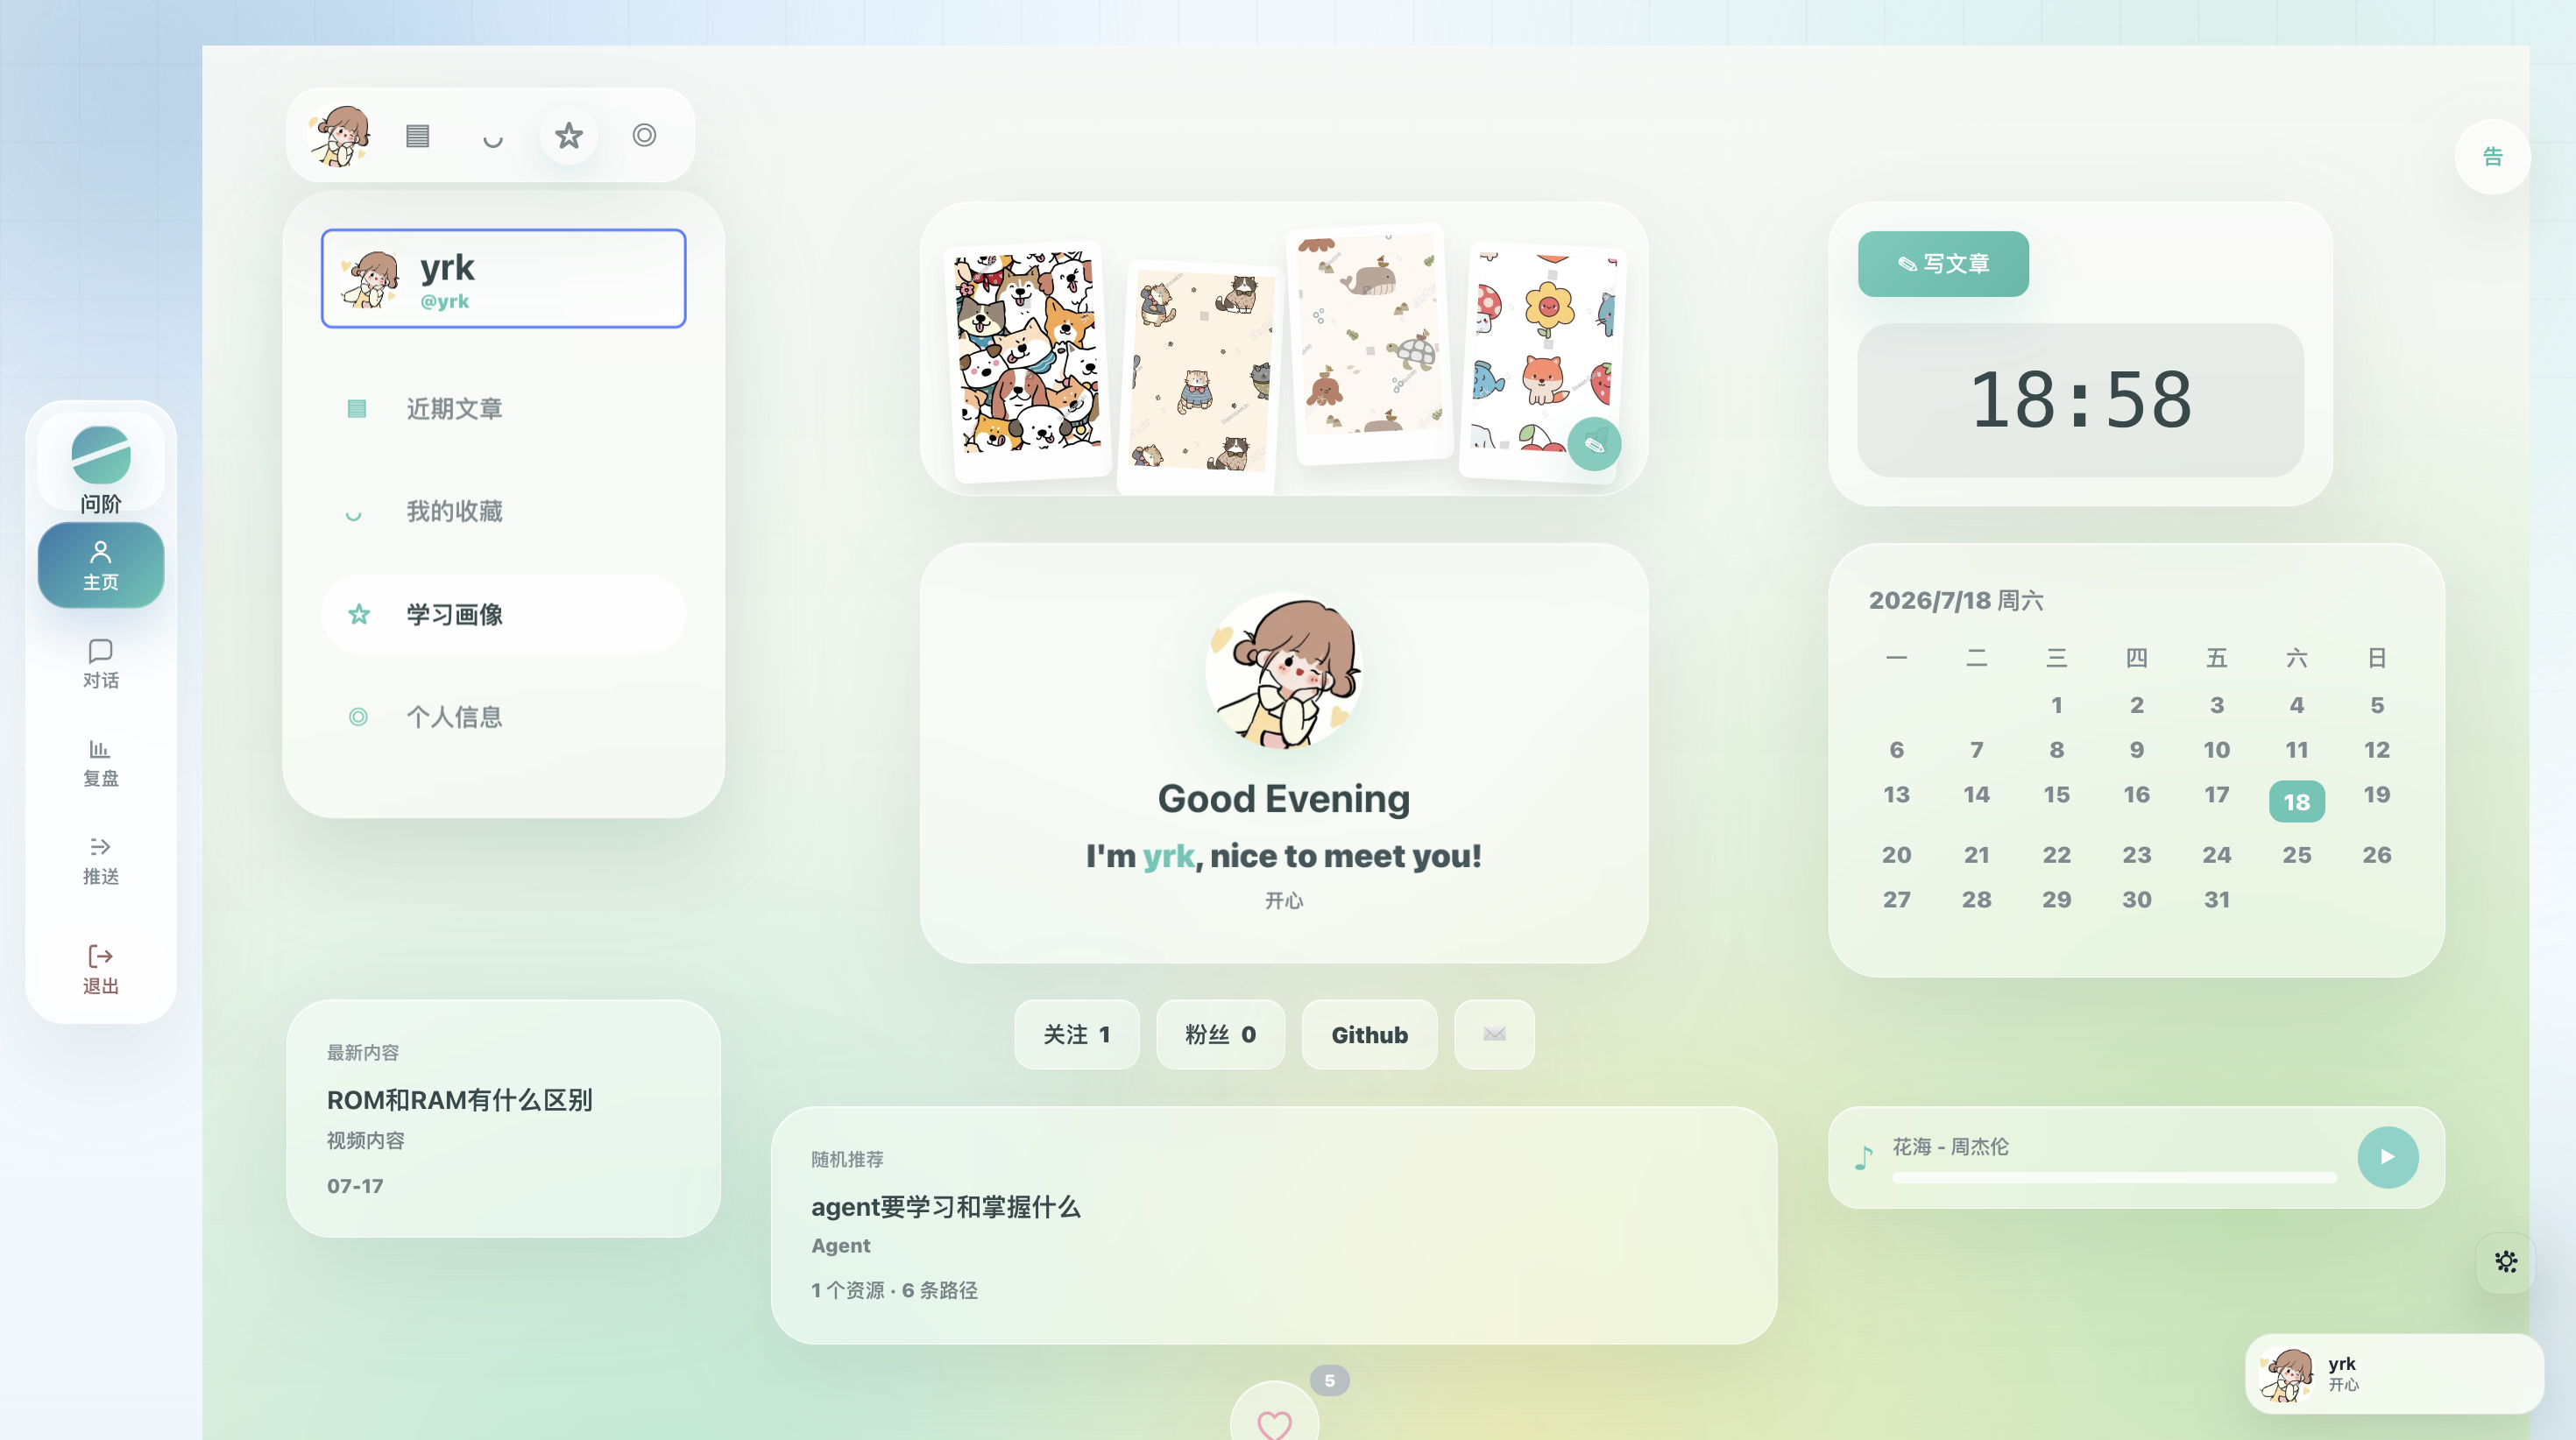
\includegraphics[width=.82\linewidth]{product-home.png}
\vspace{3mm}
\bigmetric{四个}{主入口贯通学习前、中、后}{maincolor}\hfill
\bigmetric{一个}{个人中心聚合画像与内容}{accentblue}\hfill
\bigmetric{持续}{根据近期行为给出建议}{accentred}
\end{frame}

\begin{frame}{学习画像：用户主动确认，学习行为持续补充}
\begin{columns}[T,onlytextwidth]
\column{.29\textwidth}
\vspace{5mm}
{\color{maincolor}\fontsize{29}{31}\selectfont\bfseries 8/8}\par
{\large\bfseries 维度可见、可完善}
\par\vspace{5mm}
{\small 专业·基础·认知风格·目标·易错点·偏好·节奏·兴趣}
\par\vspace{5mm}
\tagbox{maincolor}{7 个轻量问题}\par\vspace{2mm}
\tagbox{accentblue}{选项 + 自由回答}\par\vspace{2mm}
\tagbox{accentred}{学习行为持续更新}
\column{.67\textwidth}

\includegraphics[width=\linewidth]{product-profile-dialog.png}
\vspace{2mm}
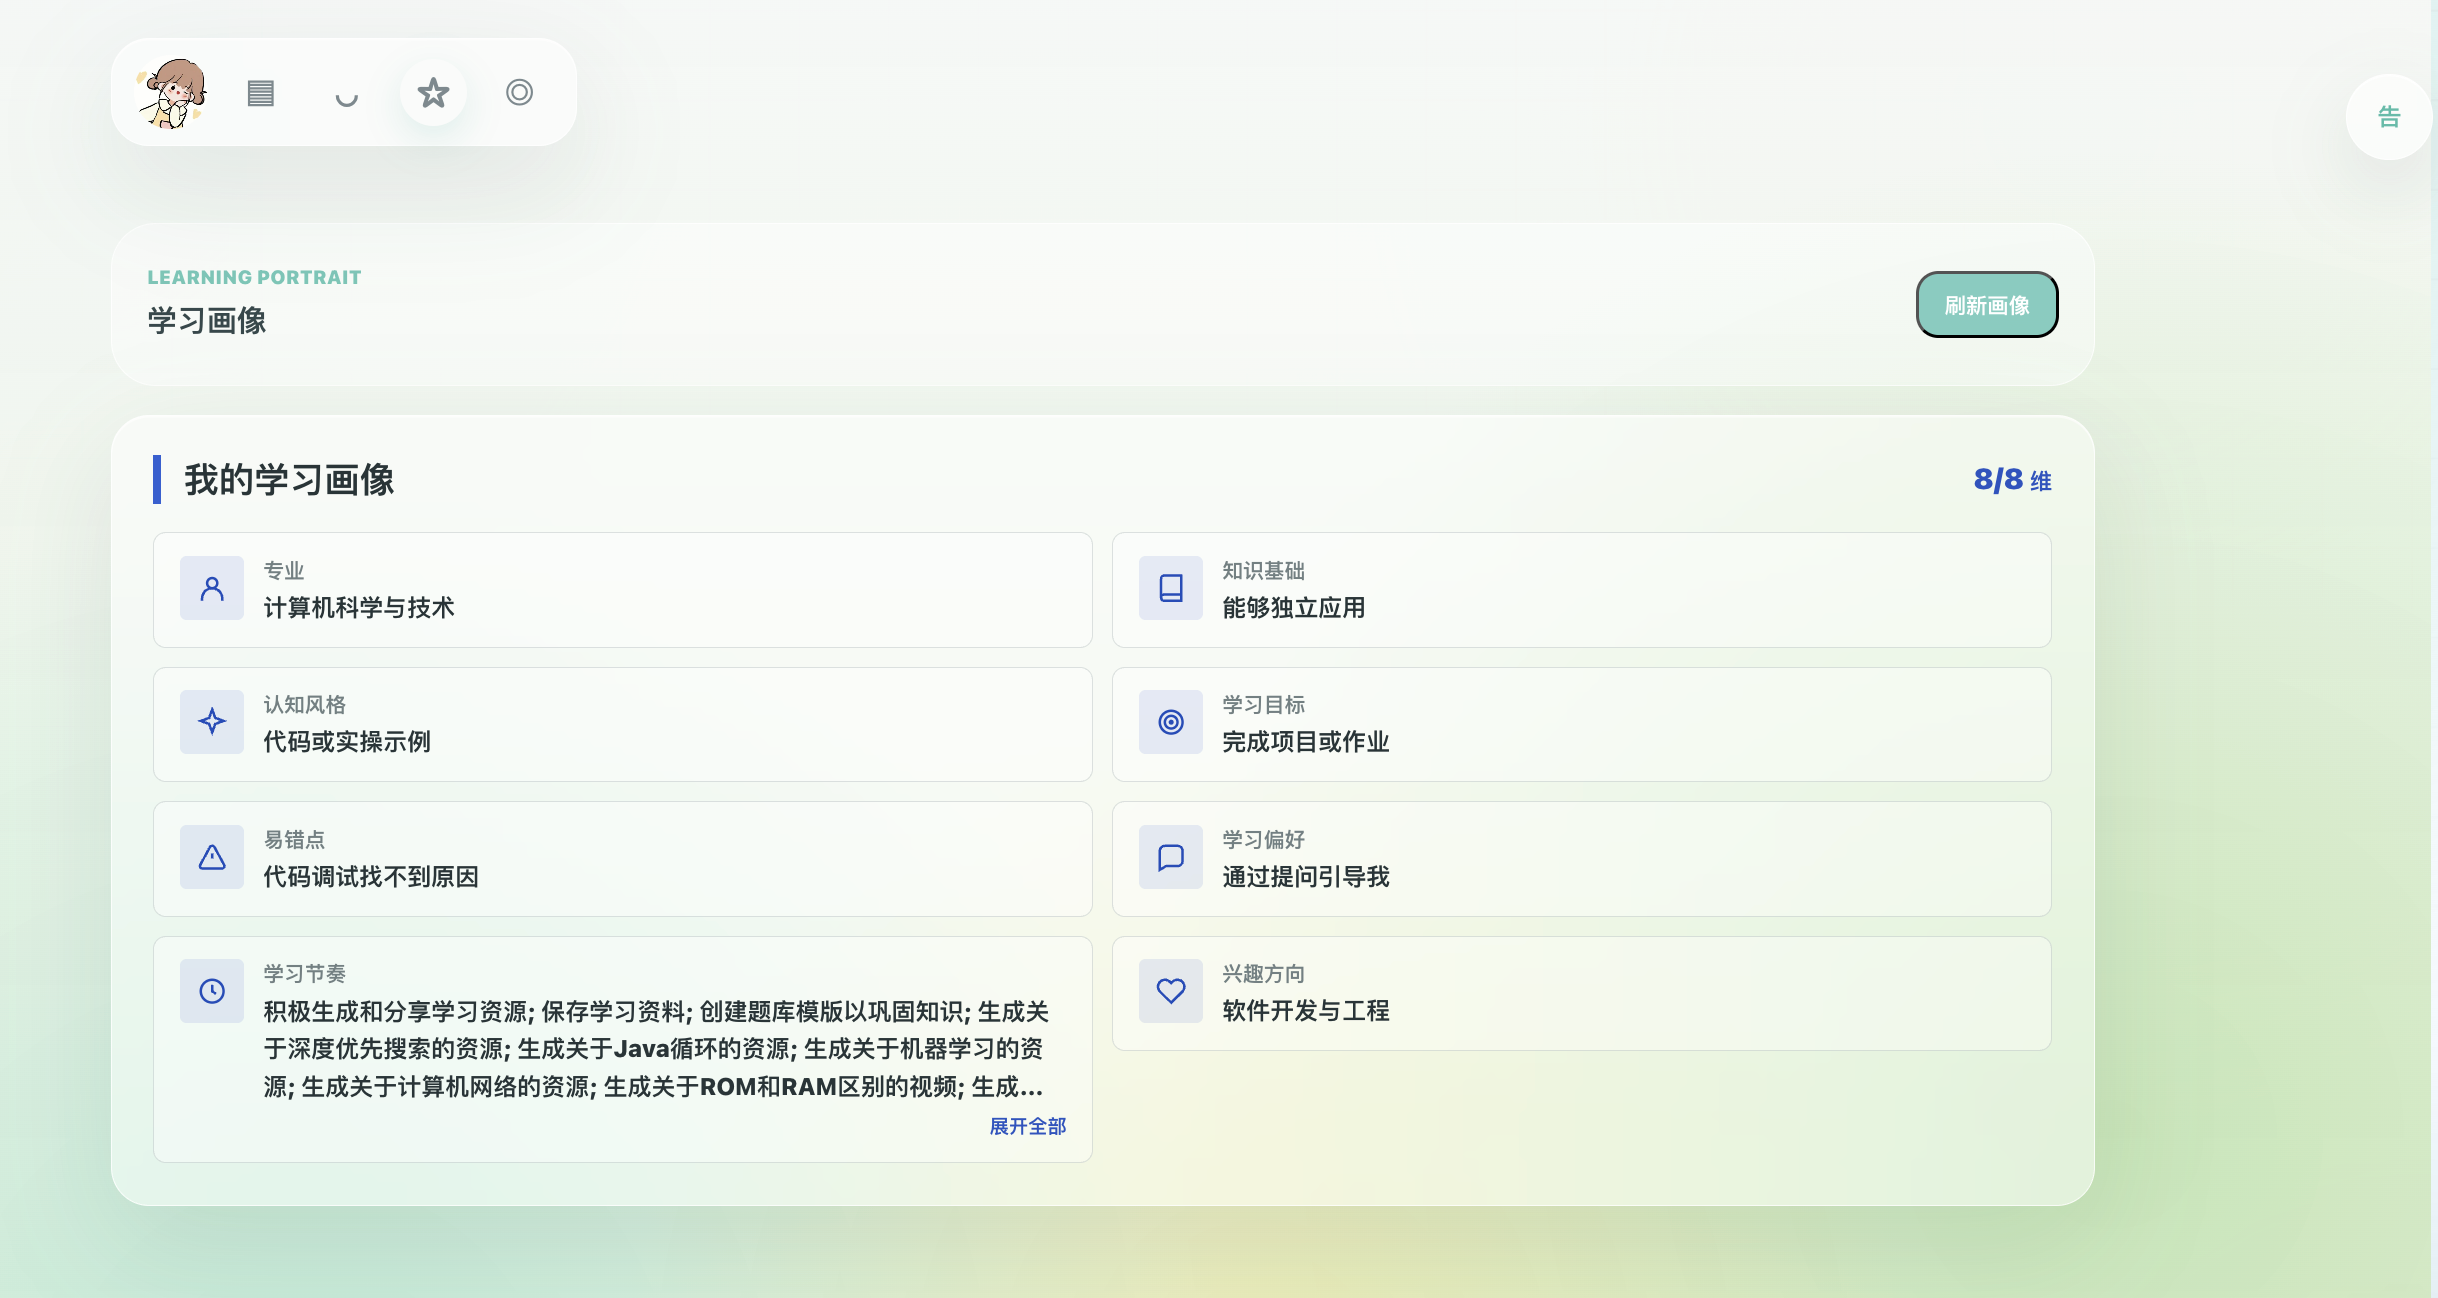
\includegraphics[width=\linewidth]{product-profile-complete.png}
\end{columns}
\end{frame}

\begin{frame}{实时答疑：一次对话同时读取学习画像与课程依据}
\centering
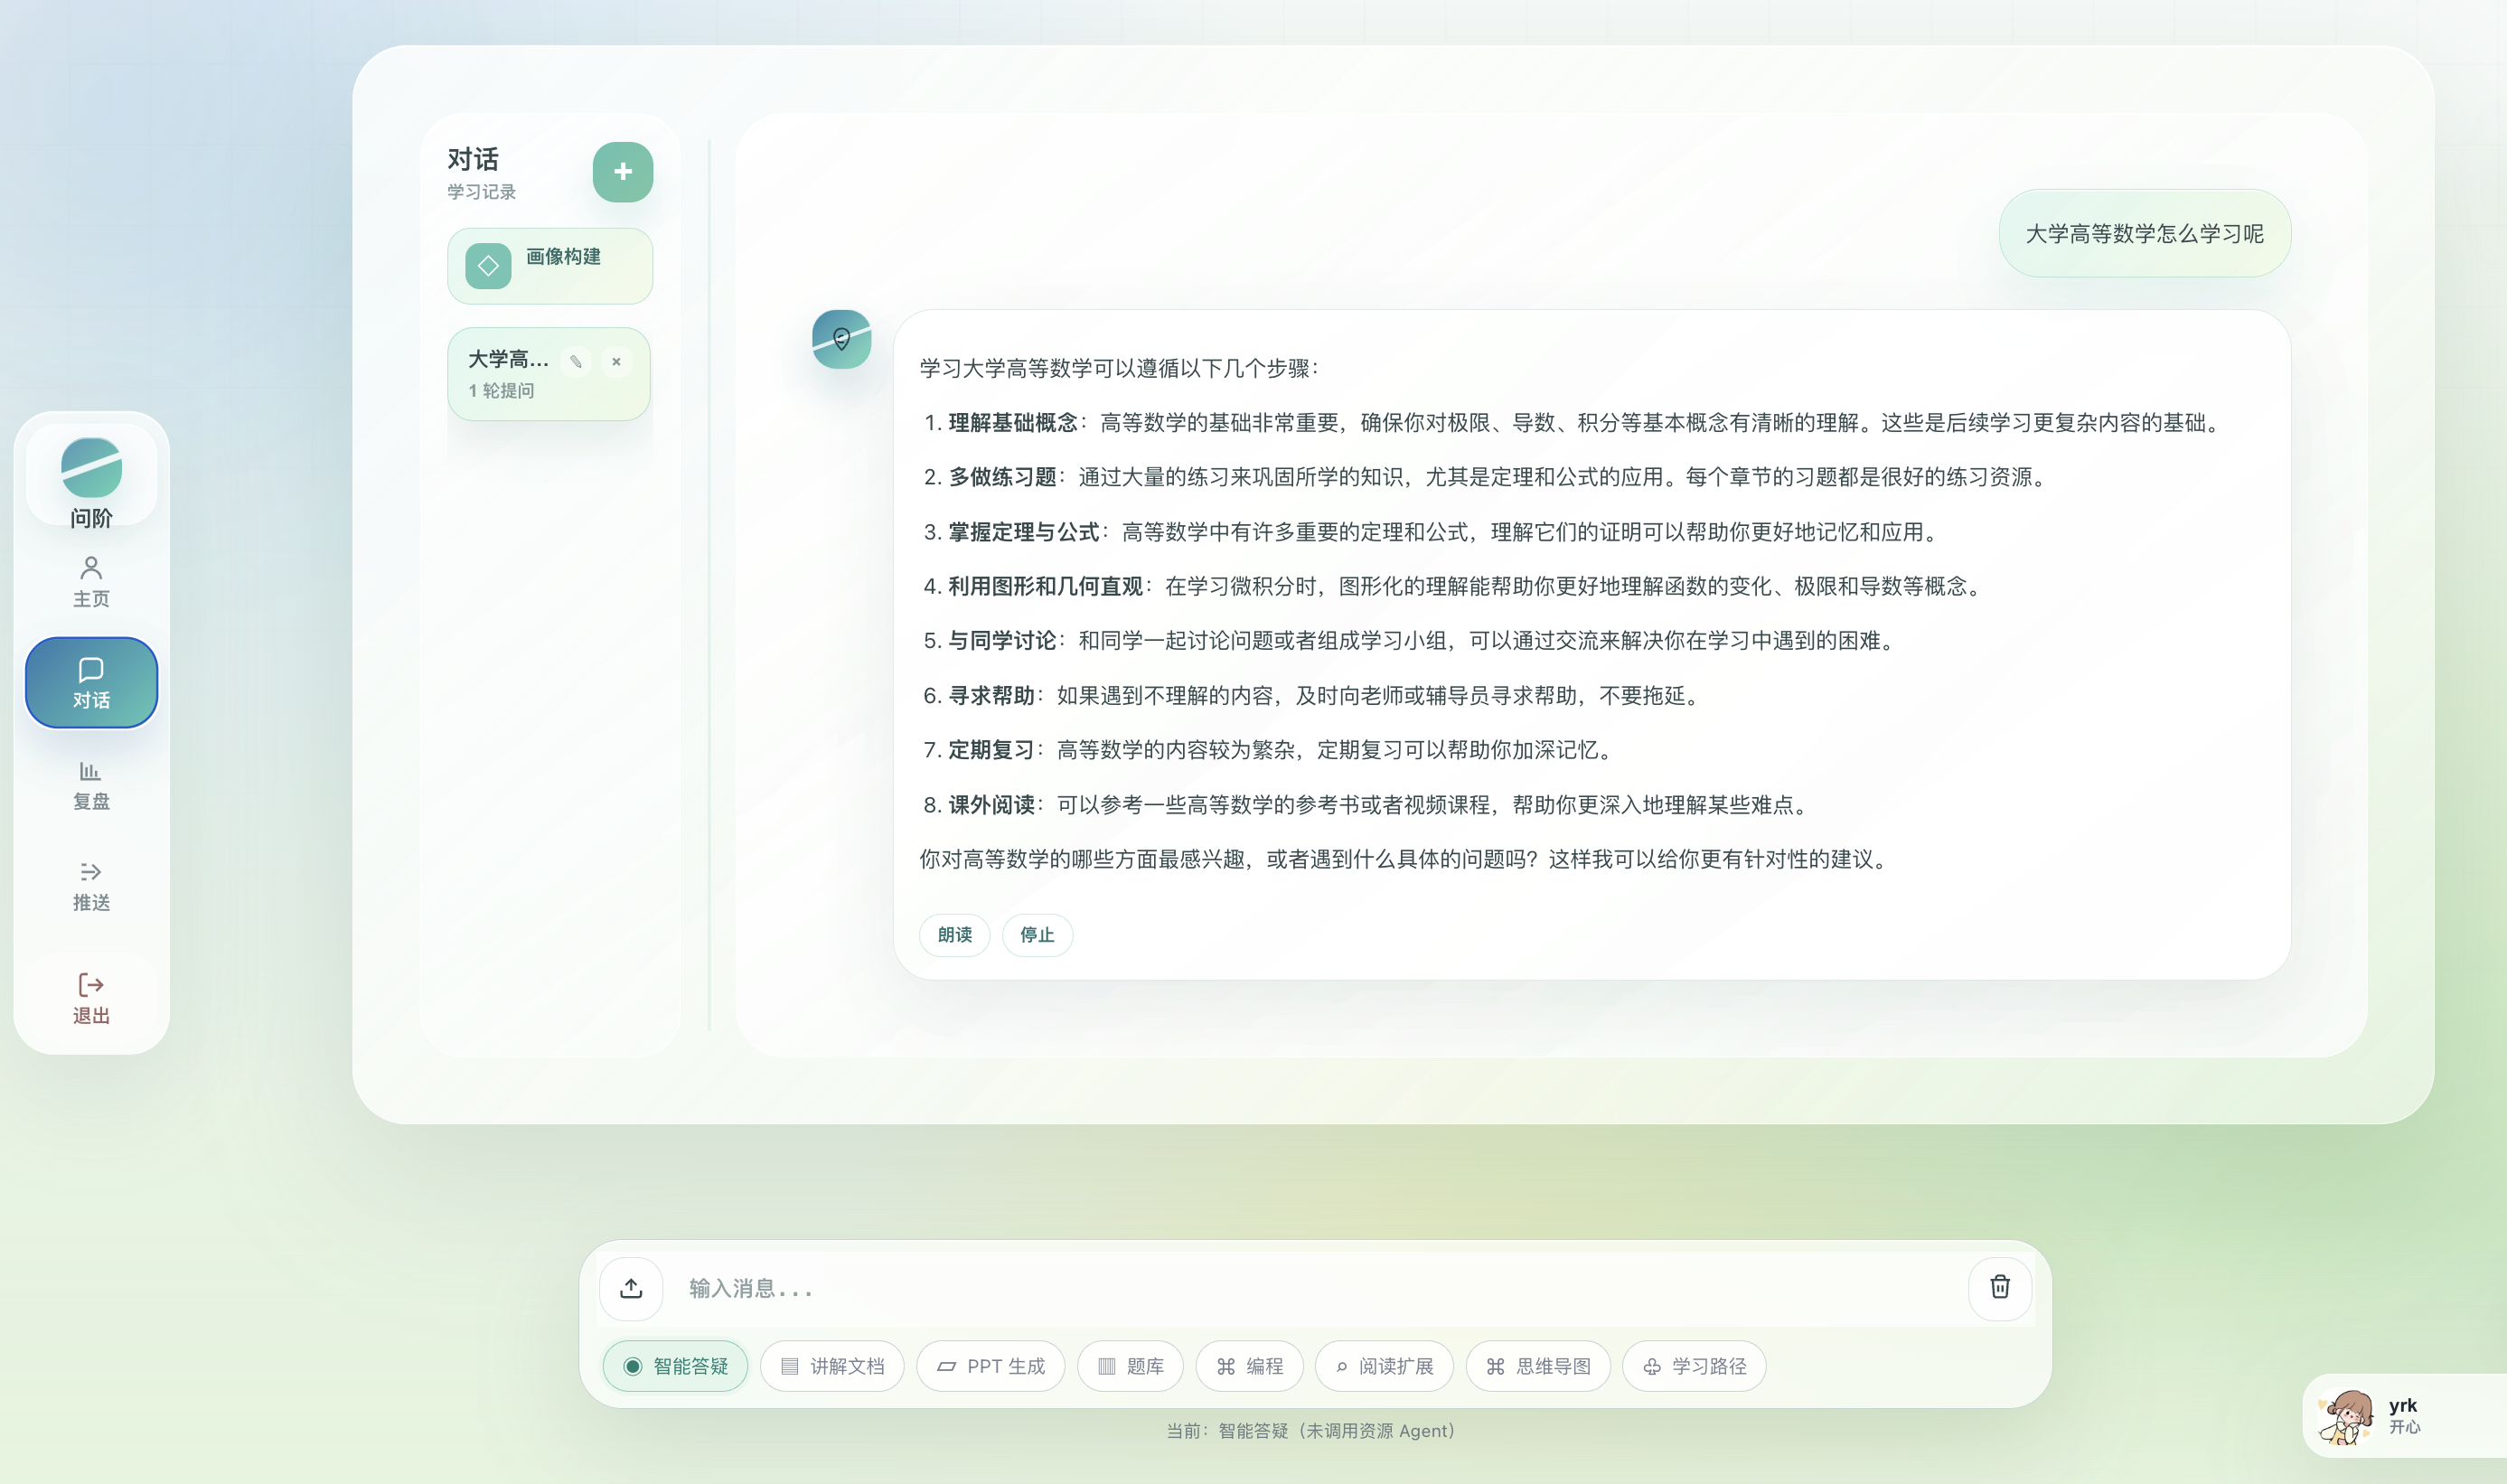
\includegraphics[width=.86\linewidth]{product-chat-live.png}
\vspace{3mm}
\begin{columns}[T,onlytextwidth]
\column{.31\textwidth}\centering
{\color{maincolor}\large\bfseries 即时交互}\par
{\scriptsize 流式回答·Markdown·代码}
\column{.31\textwidth}\centering
{\color{accentblue}\large\bfseries 对话可持续}\par
{\scriptsize 独立保存·重命名·继续追问}
\column{.31\textwidth}\centering
{\color{accentred}\large\bfseries 回答有依据}\par
{\scriptsize 补充可靠资源}
\end{columns}
\end{frame}

\begin{frame}{七类学习任务：同一对话入口完成不同形式交付}
\begin{columns}[T,onlytextwidth]
\column{.49\textwidth}
\centering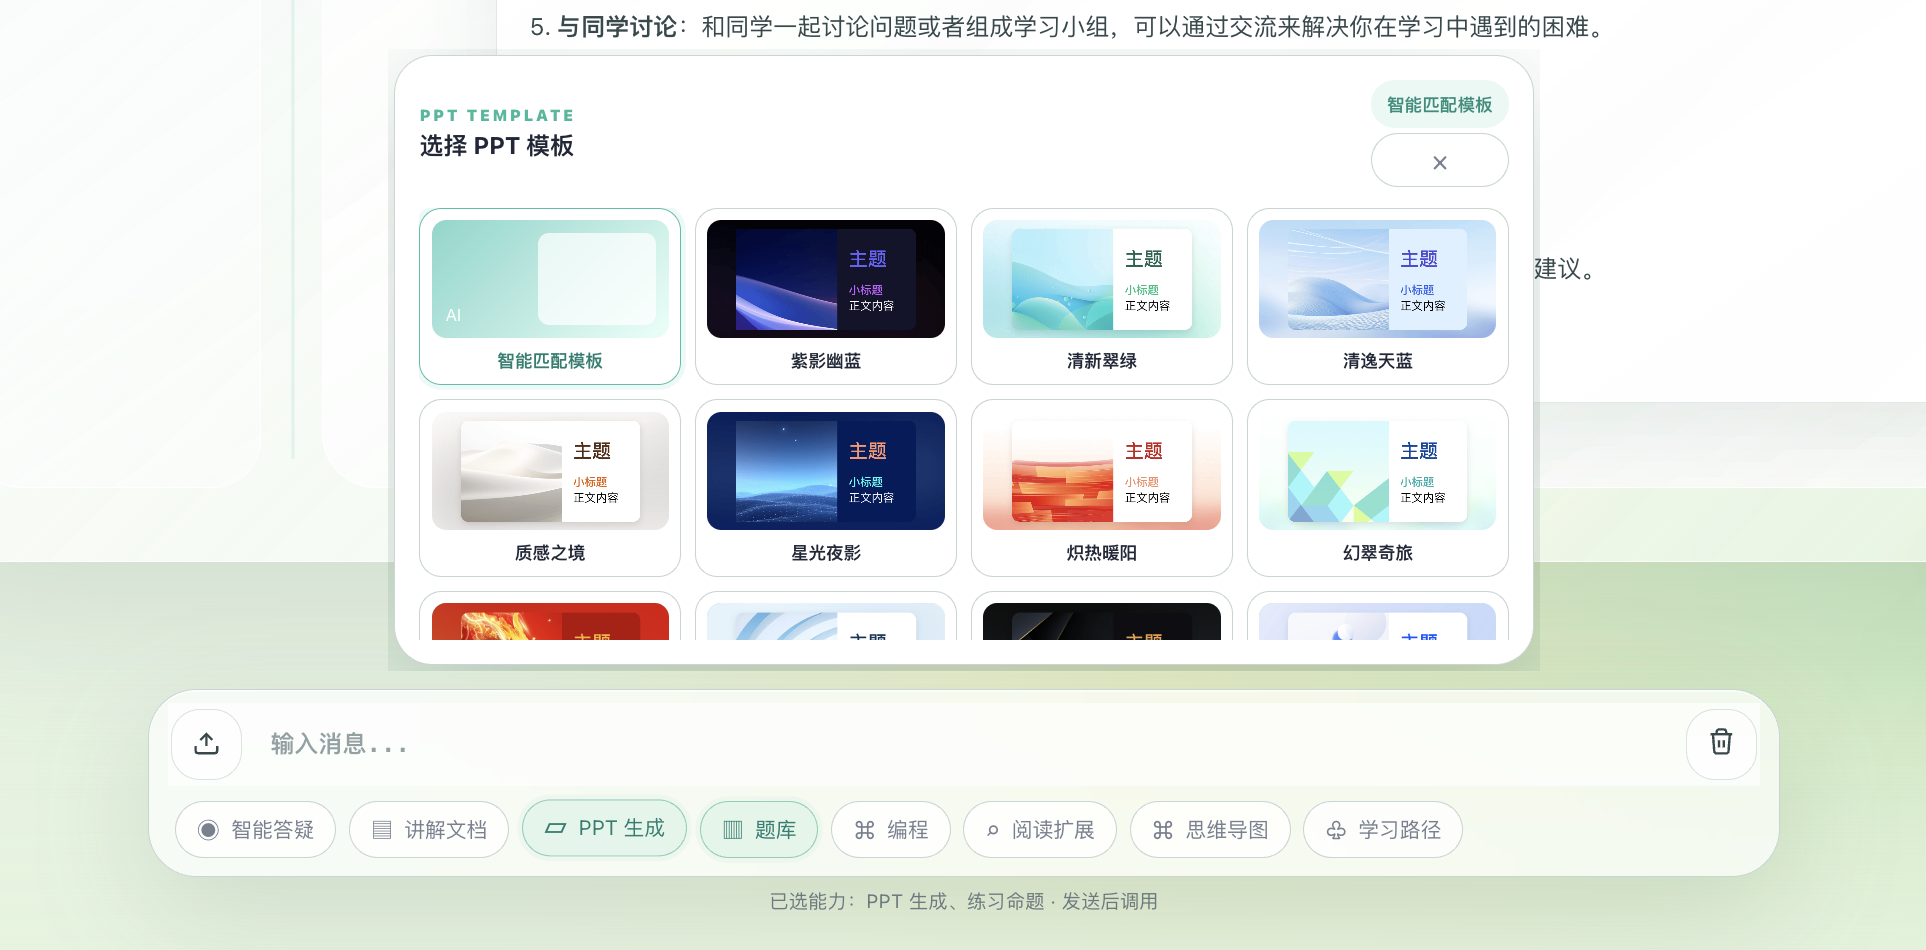
\includegraphics[width=\linewidth]{product-ppt-template.png}\par
\scriptsize PPT 根据内容智能匹配模板
\column{.49\textwidth}
\centering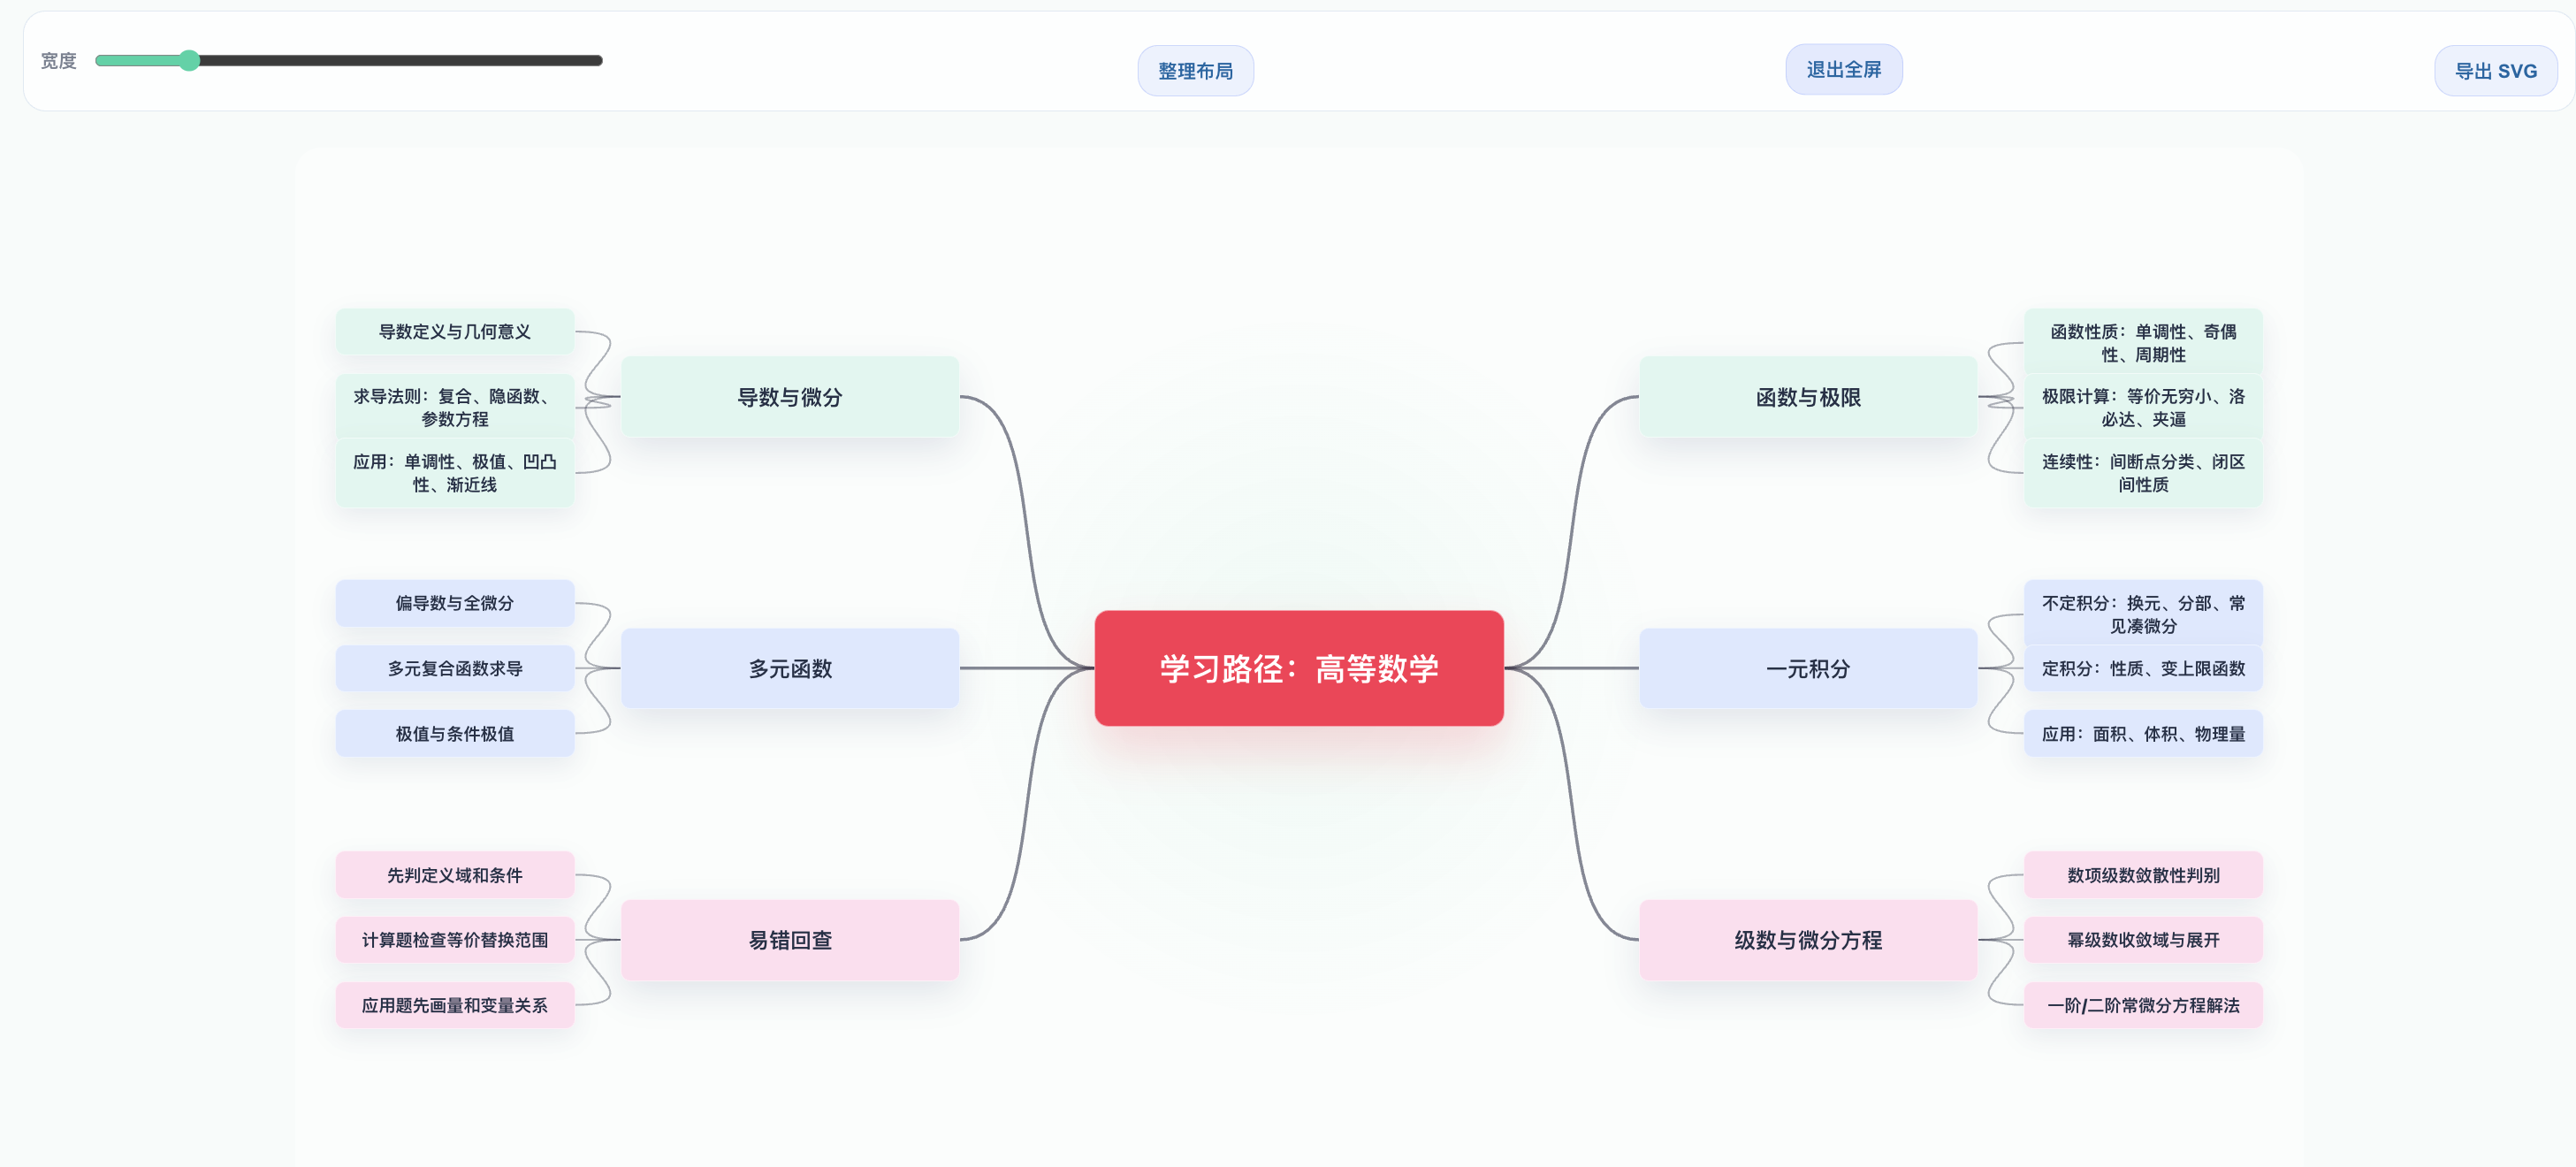
\includegraphics[width=\linewidth]{product-mindmap.png}\par
\scriptsize 思维导图将知识组织为可导出结构
\end{columns}
\vspace{1mm}
\begin{center}
\tagbox{maincolor}{讲解文档}\quad\tagbox{accentblue}{PPT}\quad
\tagbox{accentorange}{题库}\quad\tagbox{accentred}{编程}\quad
\tagbox{maincolor}{阅读扩展}\quad\tagbox{accentblue}{思维导图}\quad
\tagbox{accentgreen}{学习路径}
\end{center}
\vspace{2mm}
{\small\bfseries 需求分析 → 资源 Agent 并行生成 → 审核 Agent 整合 → 下载、保存或进入路径}
\end{frame}

\begin{frame}{学习路径：从全局总览落到可执行步骤}
\begin{columns}[T,onlytextwidth]
\column{.61\textwidth}
\centering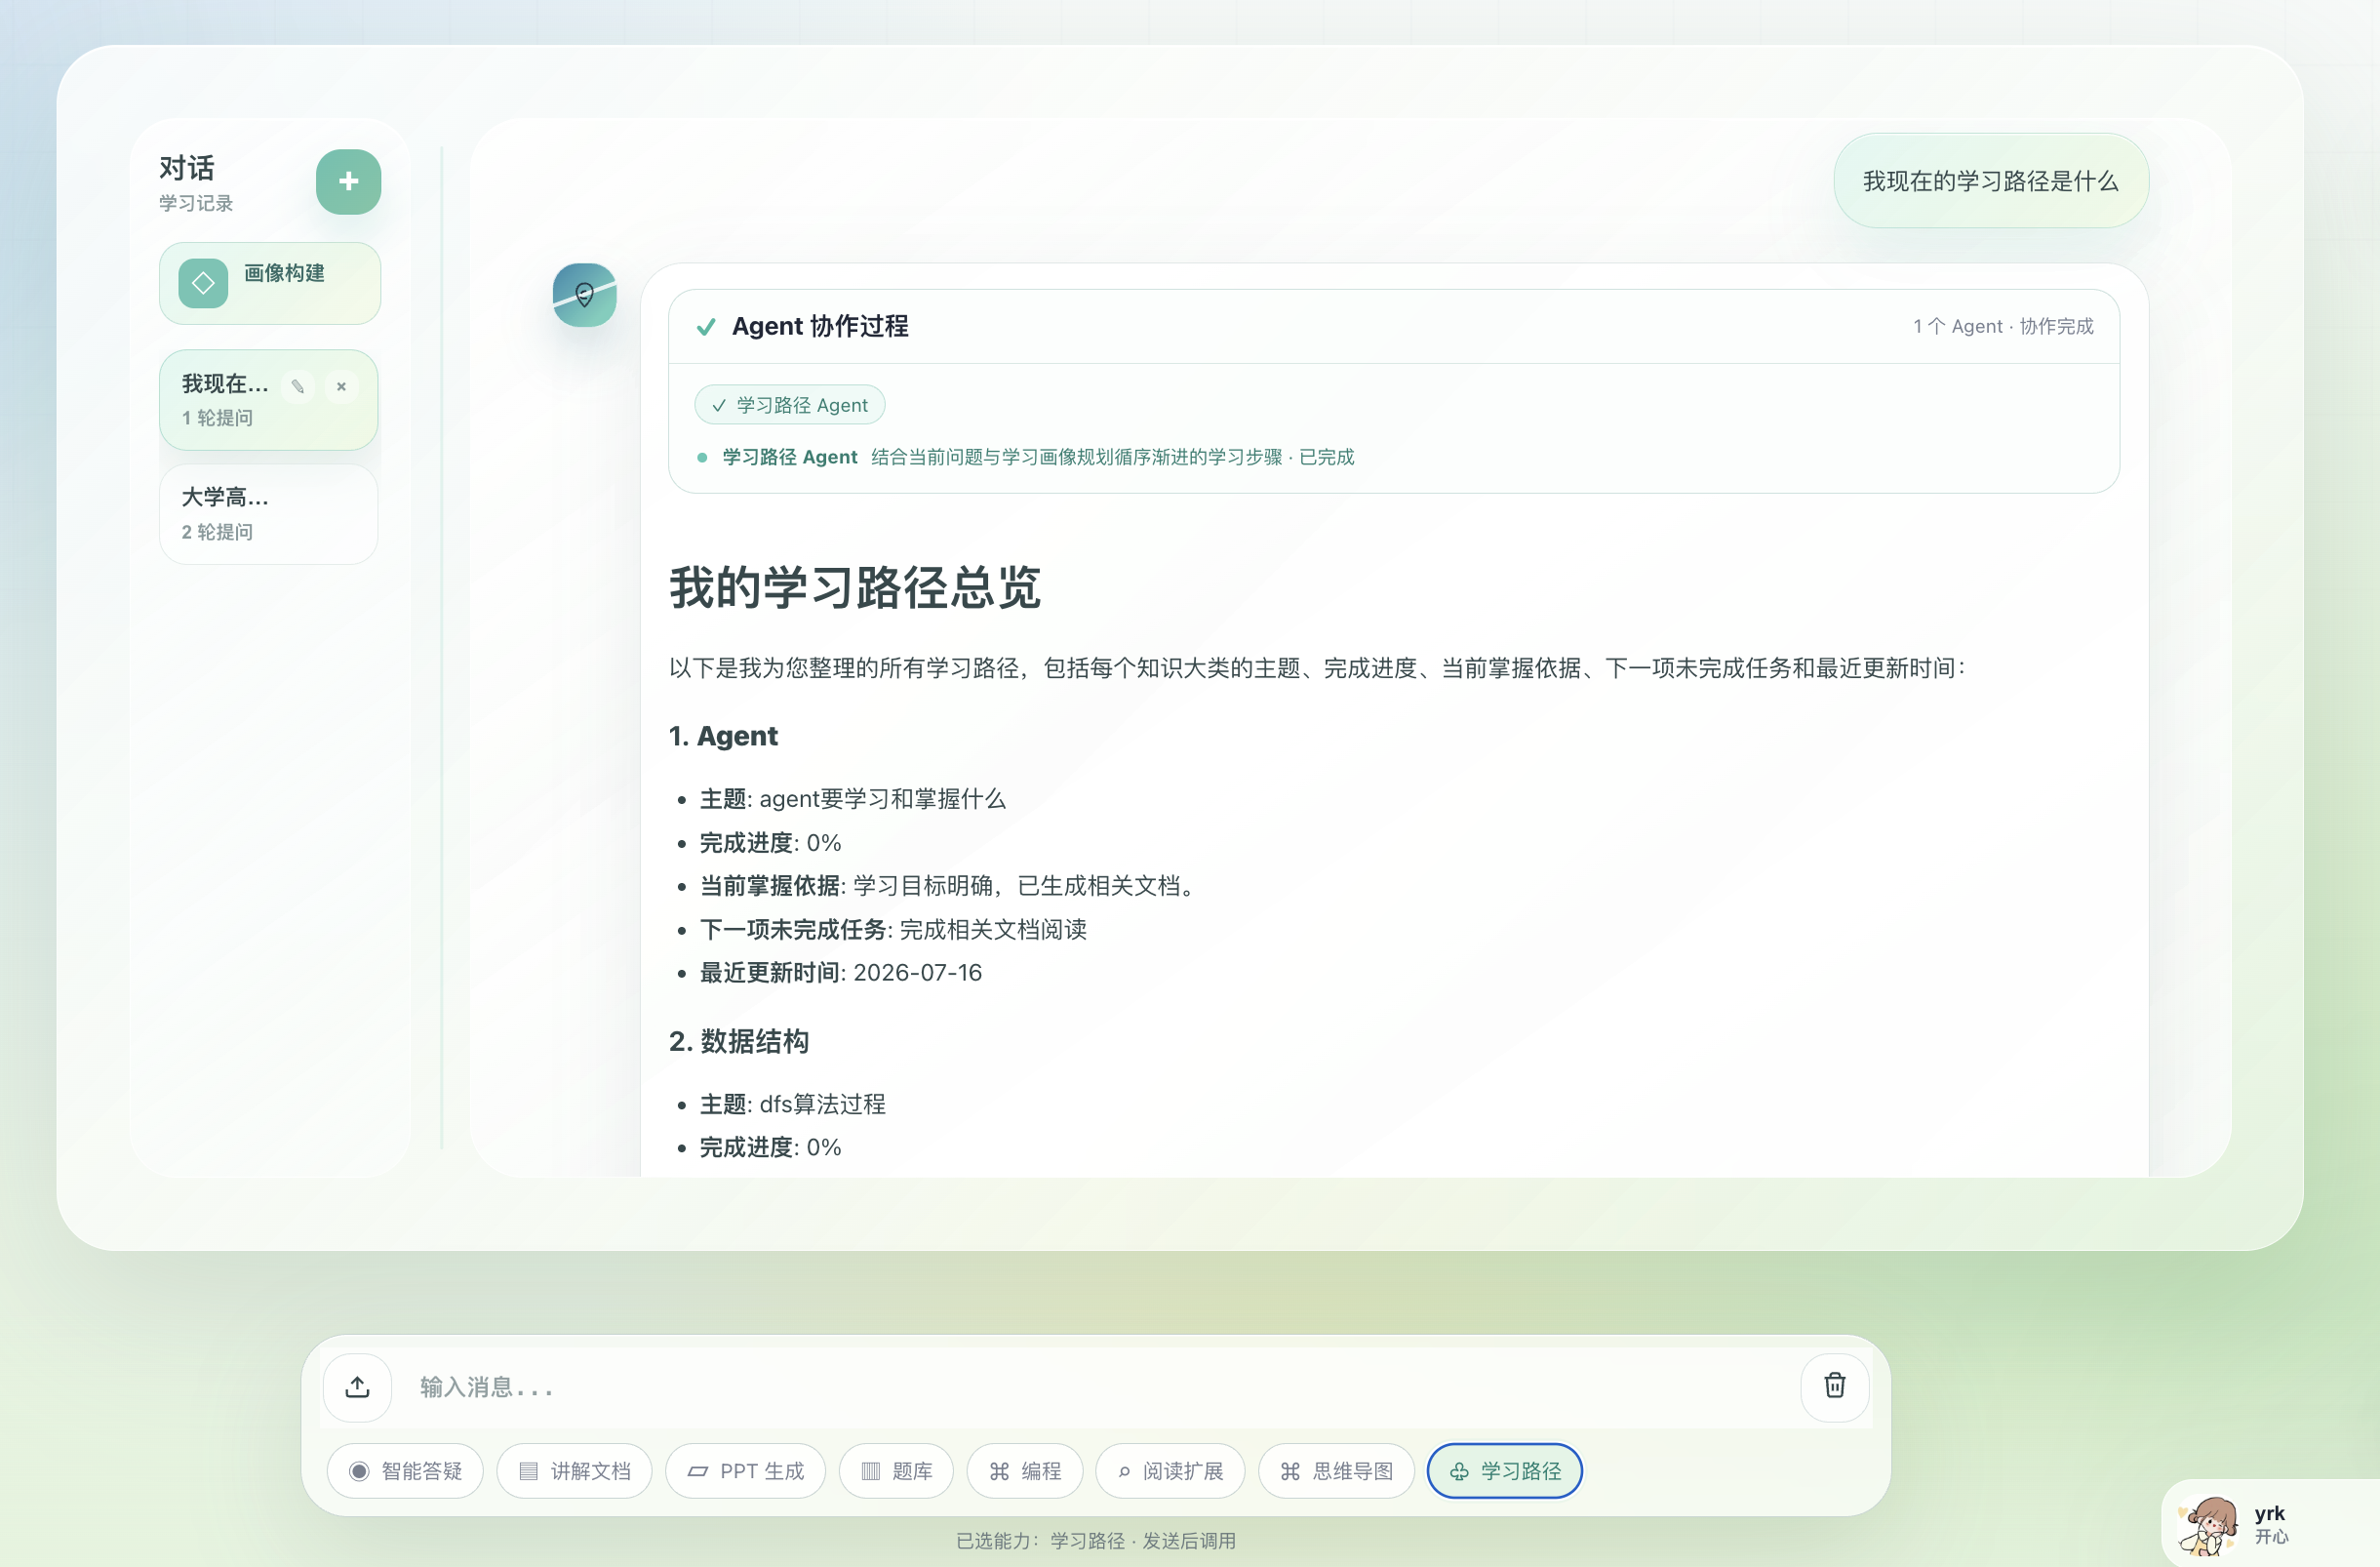
\includegraphics[width=\linewidth]{product-path-summary.png}\par
\scriptsize 路径 Agent 统一汇总主题、进度与下一项任务
\column{.36\textwidth}
\centering
\includegraphics[width=\linewidth]{product-path-steps.png}\par
\scriptsize 每个阶段给出时长、步骤与完成标准
\end{columns}
\vspace{4mm}
\begin{center}
\tagbox{maincolor}{进度可见}\quad
\tagbox{accentblue}{步骤可勾选}\quad
\tagbox{accentred}{完成标准明确}
\end{center}
\end{frame}

\begin{frame}{复盘评估：把学习行为转化为下一轮建议}
\centering
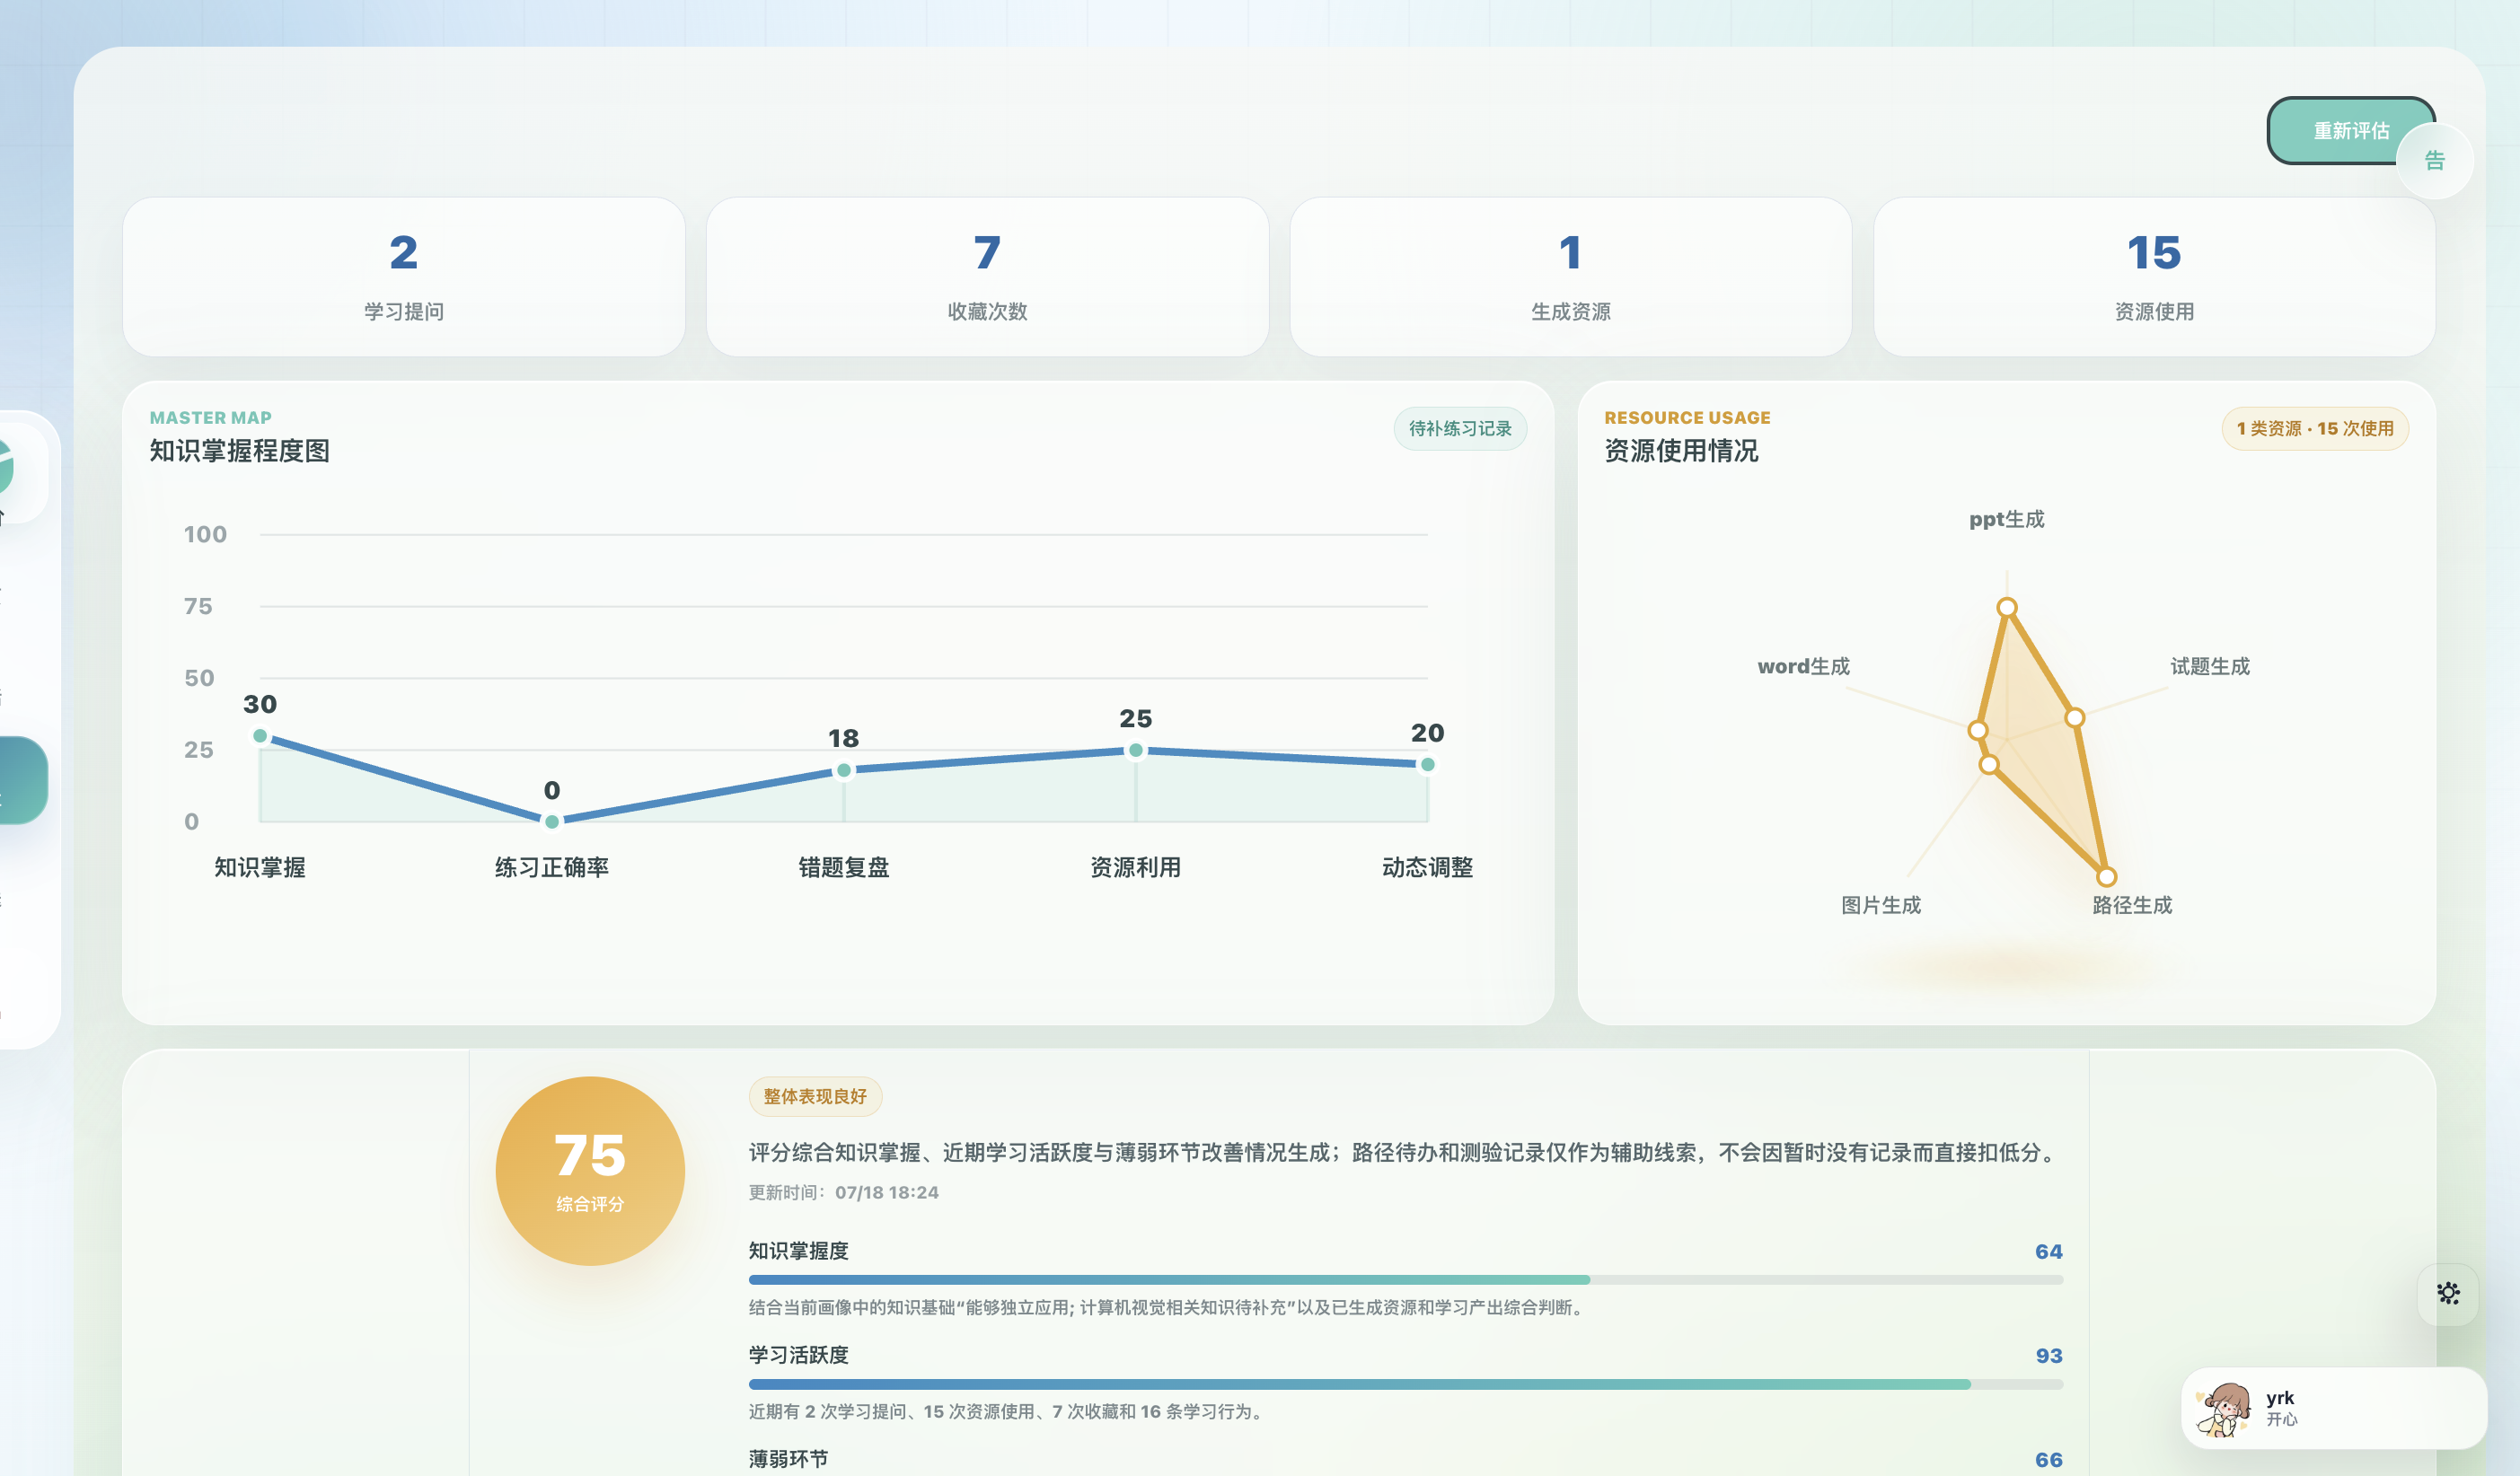
\includegraphics[width=.83\linewidth]{product-assessment.png}
\vspace{3mm}
\bigmetric{掌握}{知识理解与练习证据}{maincolor}\hfill
\bigmetric{活跃}{提问、收藏与资源使用}{accentblue}\hfill
\bigmetric{补强}{薄弱环节驱动下一轮推荐}{accentred}
\end{frame}

\begin{frame}{从个人学习到社区共享：优质内容可沉淀、可再利用}
\begin{columns}[T,onlytextwidth]
\column{.49\textwidth}
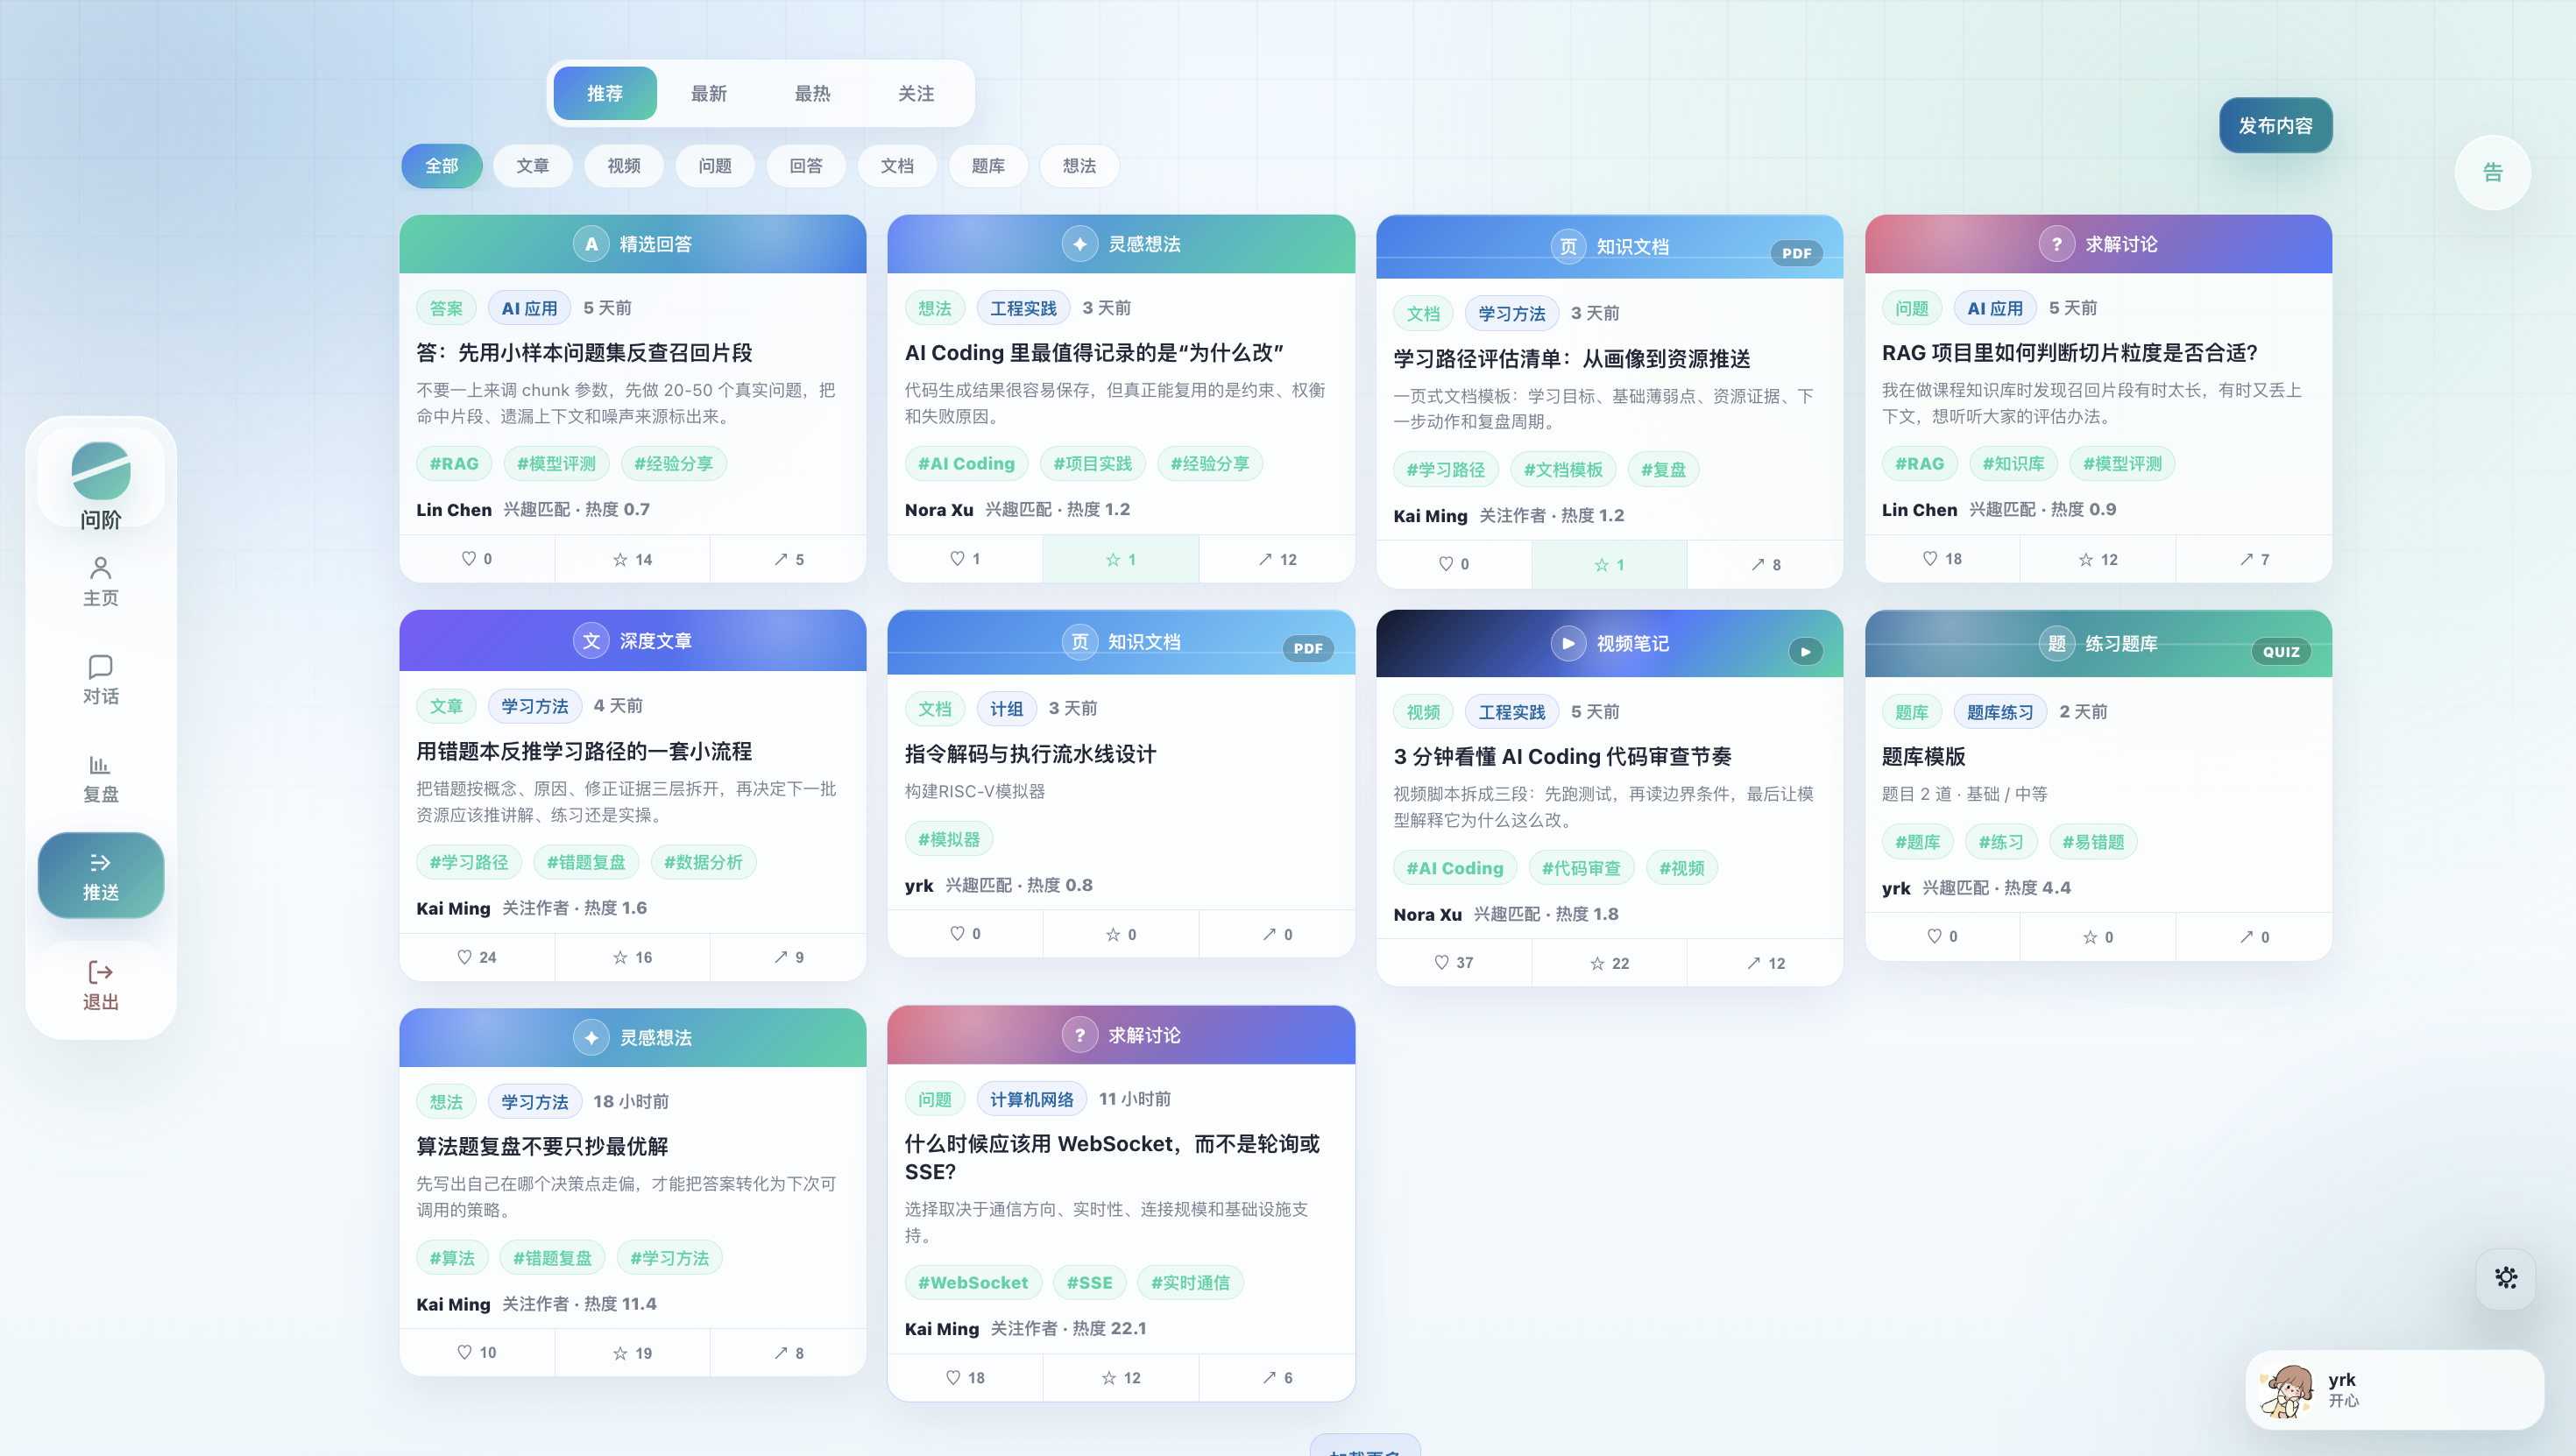
\includegraphics[width=\linewidth]{product-community.png}\par
\centering\scriptsize 推荐流汇集文章、问答、题库、视频与文档
\column{.49\textwidth}

\includegraphics[width=\linewidth]{product-article-detail.png}\par
\centering\scriptsize 长文内容保留目录、代码与作者信息
\end{columns}
\vspace{3mm}
\begin{beamercolorbox}[wd=\textwidth,sep=2.5mm,center,rounded=true]{block body}
{\small\bfseries AI 生成 / 可信检索 → 收藏、编辑与归类 → 社区发布 → 使用反馈进入推荐}
\end{beamercolorbox}
\end{frame}

\begin{frame}{响应式交互：同一学习闭环覆盖电脑与移动端}
\begin{columns}[T,onlytextwidth]
\column{.31\textwidth}
\centering
\includegraphics[height=5.55cm]{product-mobile-home.png}\par
\scriptsize 个人首页与底部导航
\column{.31\textwidth}
\centering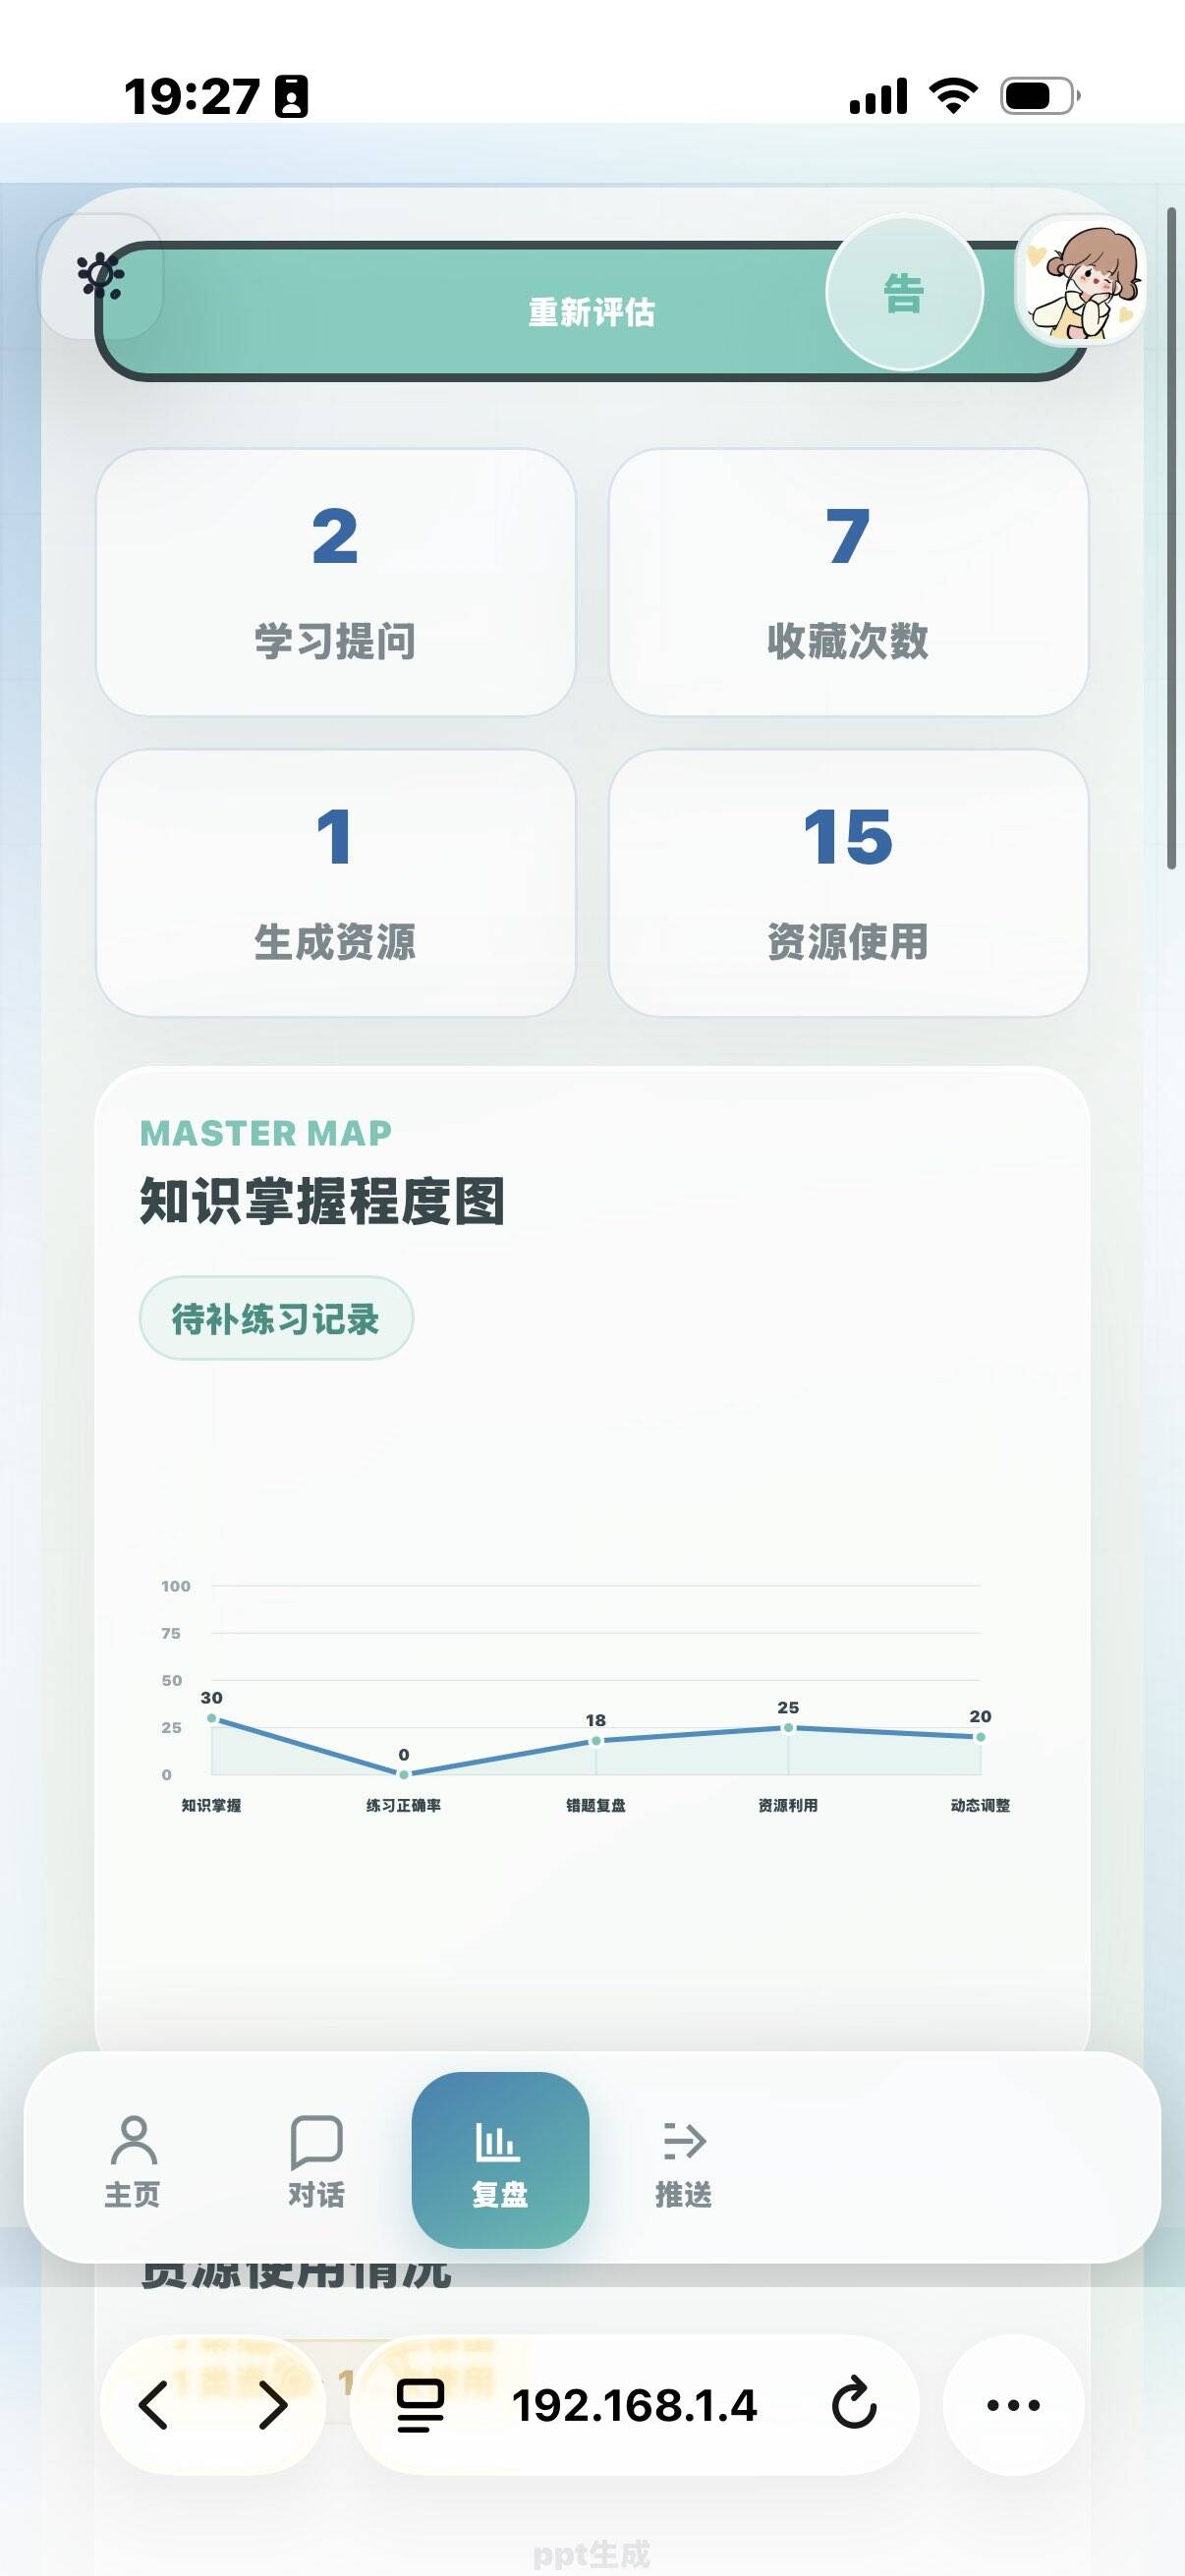
\includegraphics[height=5.55cm]{product-mobile-review.png}\par
\scriptsize 复盘数据与掌握趋势
\column{.31\textwidth}
\centering
\includegraphics[height=5.55cm]{product-mobile-community.png}\par
\scriptsize 社区内容与分类浏览
\end{columns}
\vspace{2mm}
\begin{center}
\tagbox{maincolor}{底部四导航}\quad
\tagbox{accentblue}{单栏自适应}\quad
\tagbox{accentred}{触控友好}
\end{center}
\end{frame}

\section{关键技术}

\begin{frame}{画像与动态路径：用户确认起点，行为持续校准}
\begin{columns}[T,onlytextwidth]
\column{.54\textwidth}
\centering
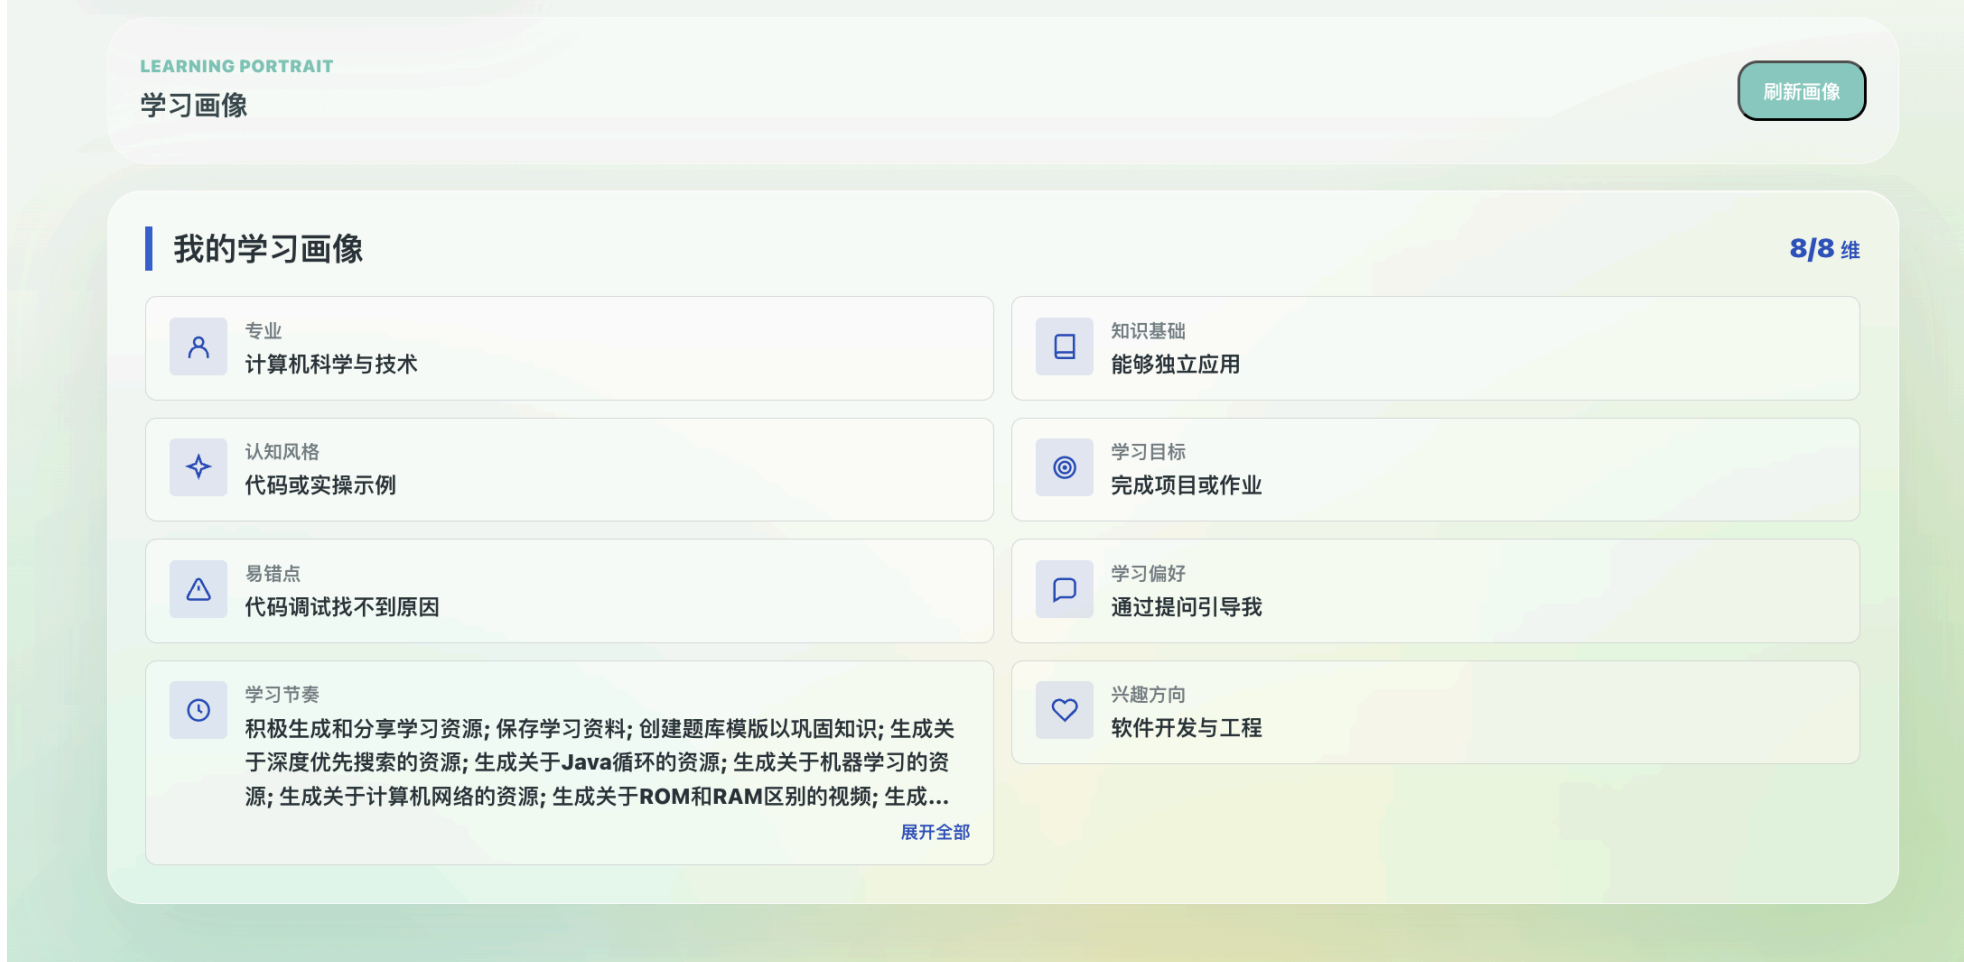
\includegraphics[width=\linewidth]{product-profile-detail.png}\par
{\tiny 8 维画像回答“怎么教”}
\column{.42\textwidth}
\centering

\includegraphics[height=2.35cm]{product-path-steps.png}\par
{\tiny 阶段、时长与完成标准落到“下一步教什么”}
\end{columns}
\vspace{2mm}
\centering
\resizebox{.70\linewidth}{!}{%
\begin{tikzpicture}[node distance=4mm and 5mm]
\tikzset{p/.style={draw=maincolor!30,fill=maincolor!5,rounded corners=3pt,minimum width=2.35cm,minimum height=.85cm,align=center,font=\scriptsize},
pa/.style={-{Stealth[length=1.8mm]},draw=maincolor,line width=.9pt}}
\node[p](q){7 个轻量问题\\用户主动确认};
\node[p,below=of q](b){对话·错题·资源\\Todo·路径进度};
\node[p,right=8mm of q,fill=accentblue!9](m){8 维学习画像\\当前状态估计};
\node[p,right=of m,fill=accentred!9](g){阶段生成\\任务与建议};
\node[p,below=of g](e){完成证据\\下一轮更新};
\draw[pa](q)--(m);\draw[pa](b)-|(m);\draw[pa](m)--(g);\draw[pa](g)--(e);\draw[pa](e.west)-|(m.south);
\end{tikzpicture}
}
\vspace{2mm}
\begin{center}\tagbox{maincolor}{画像可解释}\quad\tagbox{accentblue}{路径可执行}\quad\tagbox{accentred}{反馈可更新}\end{center}
\end{frame}

\begin{frame}{多智能体协作：并行生成、审核整合、失败隔离}
\centering
\begin{tikzpicture}[node distance=4mm]
\tikzset{n/.style={draw=maincolor!30,fill=maincolor!5,rounded corners=3pt,minimum height=1.12cm,align=center,font=\scriptsize},
na/.style={-{Stealth[length=2mm]},draw=maincolor,line width=1pt}}
\node[n,minimum width=2.25cm](d){需求分析 Agent\\分解交付目标};
\node[n,right=of d,minimum width=3.15cm,fill=accentblue!8](r){资源 Agent 并行生成\\文档·题库·导图·路径};
\node[n,right=of r,minimum width=2.45cm,fill=accentred!8](v){审核 Agent\\格式·来源·完整性};
\node[n,right=of v,minimum width=2.25cm,fill=maincolor!12](o){统一结果池\\下载·收藏·使用};
\draw[na](d)--(r);\draw[na](r)--(v);\draw[na](v)--(o);
\end{tikzpicture}
\vspace{8mm}
\begin{columns}[T,onlytextwidth]
\column{.31\textwidth}\centering
{\color{maincolor}\LARGE\bfseries 并行执行}\par
{\scriptsize 多类资源同时生成\\缩短用户等待}
\column{.31\textwidth}\centering
{\color{accentblue}\LARGE\bfseries 45 秒}\par
{\scriptsize 单任务超时边界\\支持一次重试}
\column{.31\textwidth}\centering
{\color{accentred}\LARGE\bfseries 失败隔离}\par
{\scriptsize 局部 Agent 失败\\其他结果仍可交付}
\end{columns}
\vspace{7mm}
\begin{beamercolorbox}[wd=.88\textwidth,sep=2.3mm,center,rounded=true]{block body}
{\small\bfseries 并行保证效率，审核保证质量，失败隔离保证稳定交付。}
\end{beamercolorbox}
\end{frame}

\begin{frame}{复盘与推荐闭环：学习证据驱动下一轮行动}
\begin{columns}[T,onlytextwidth]
\column{.62\textwidth}
\vspace{6mm}
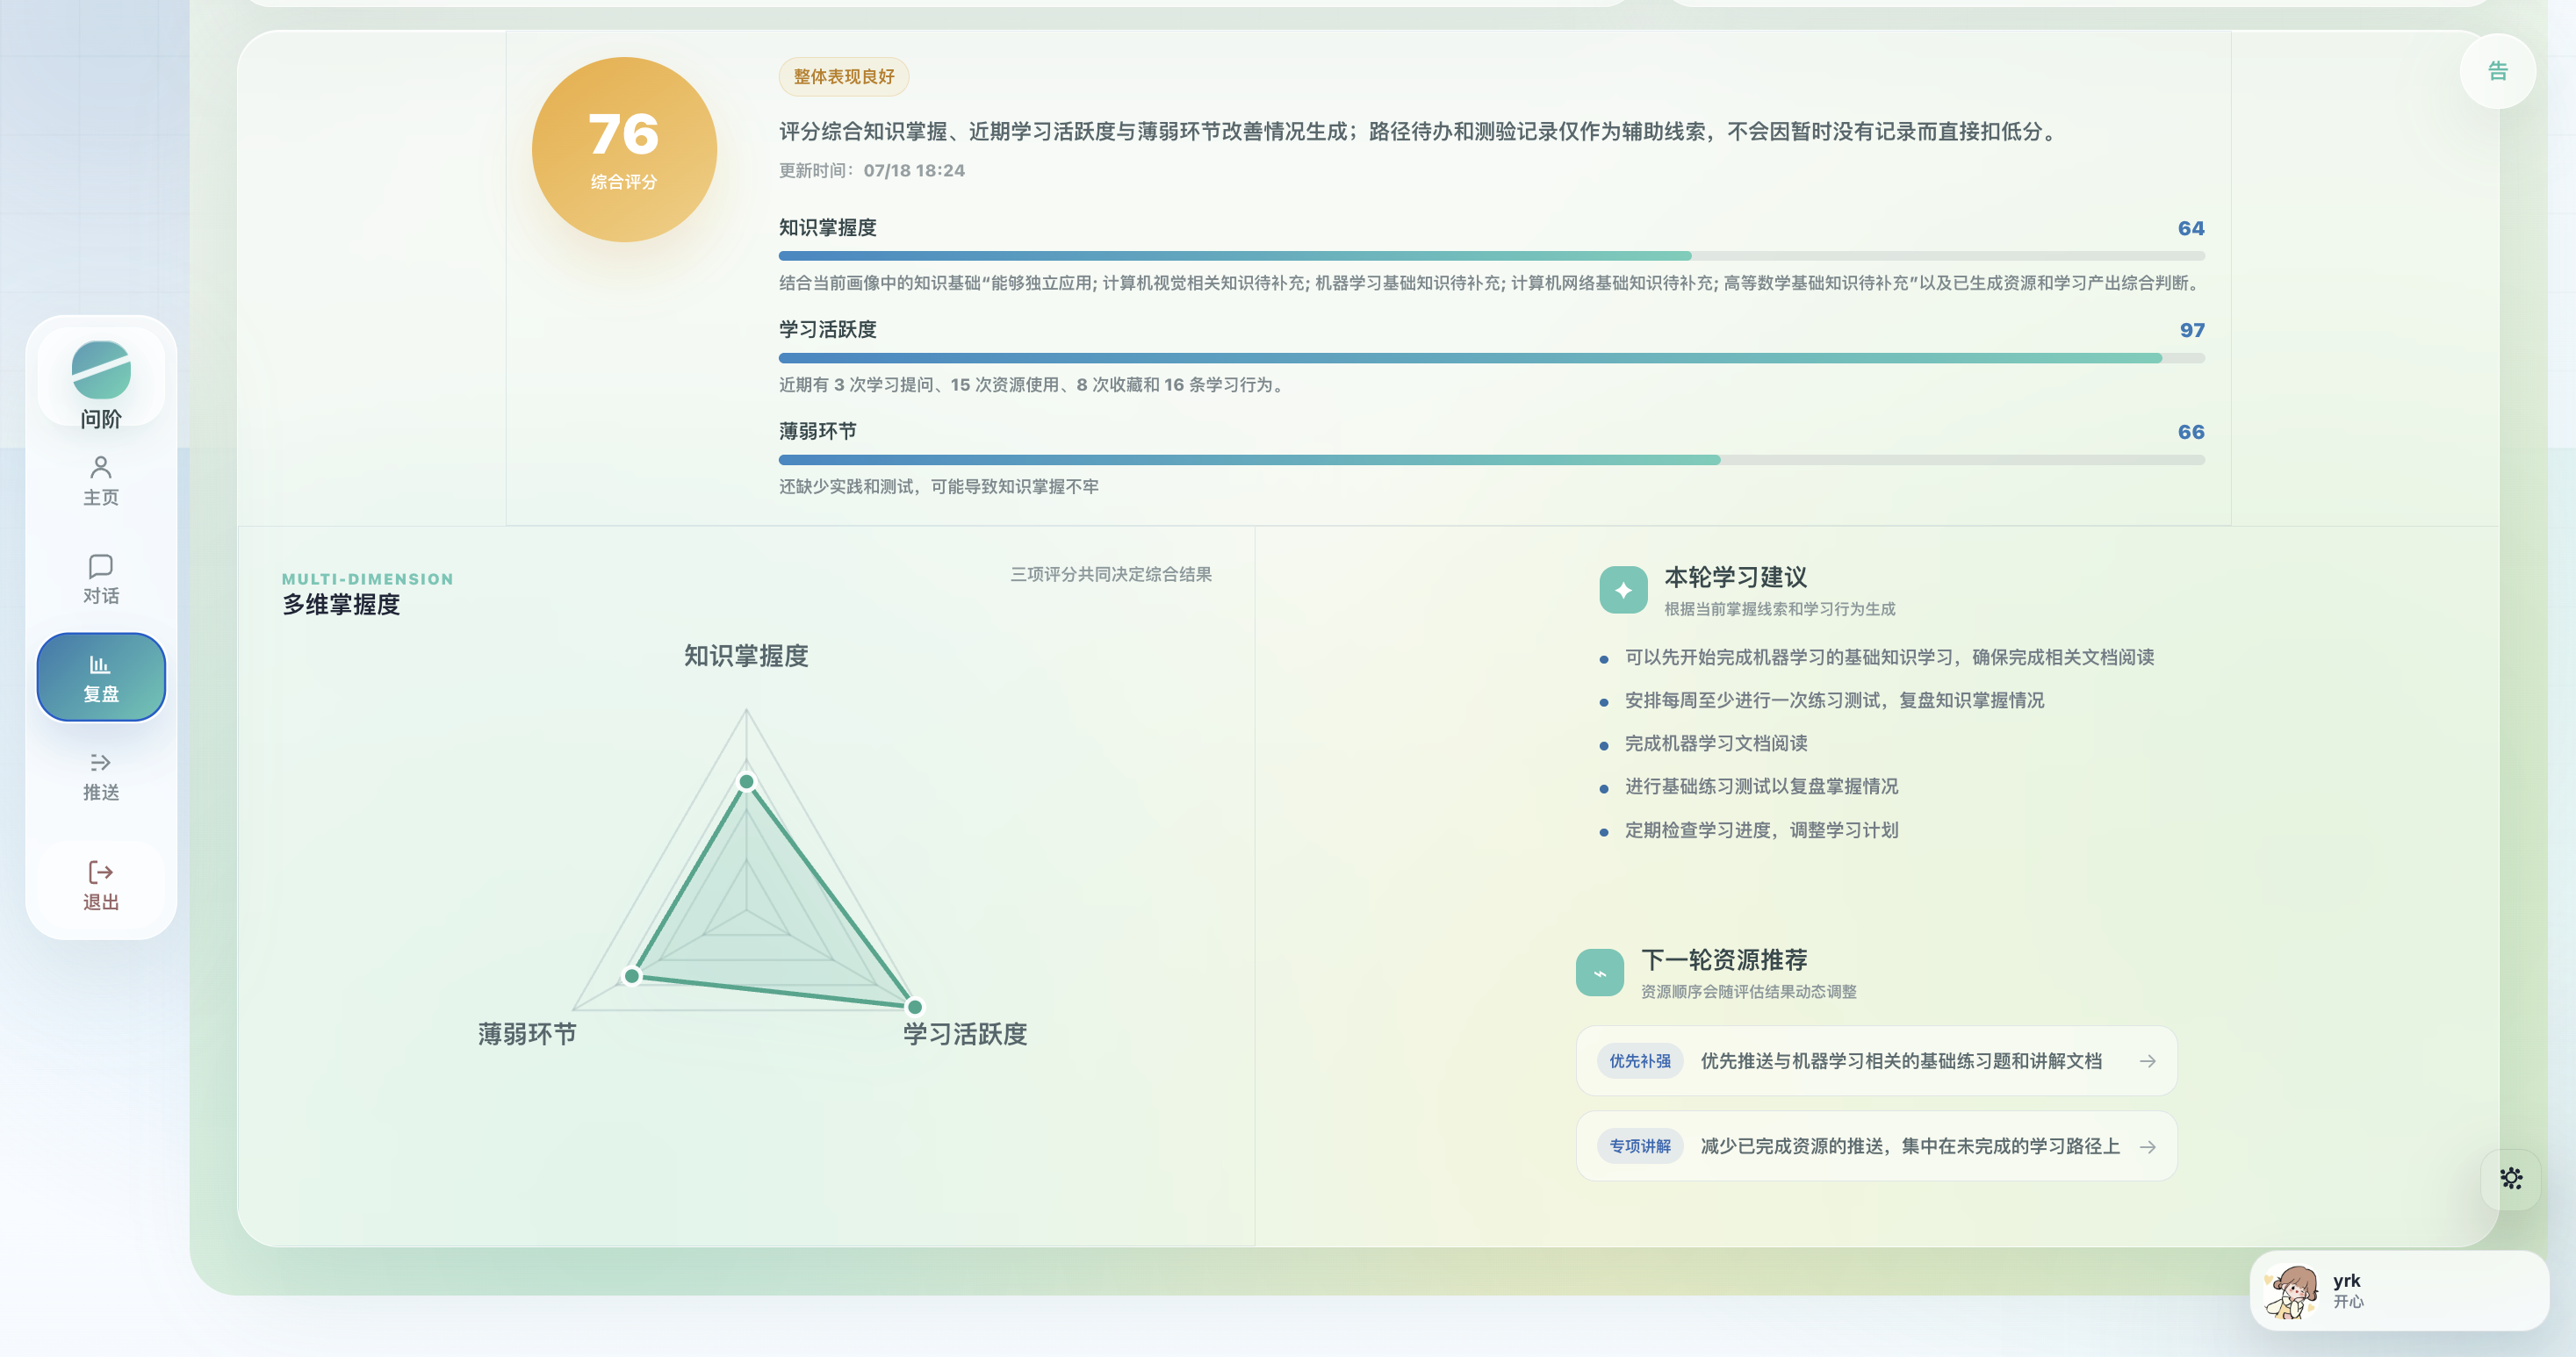
\includegraphics[width=\linewidth]{product-assessment-loop.png}
\column{.34\textwidth}
\vspace{1mm}
{\color{maincolor}\fontsize{20}{22}\selectfont\bfseries 01}\quad{\large\bfseries 聚合证据}\par
{\scriptsize\hspace{7mm}提问、收藏、资源使用、练习与 Todo}\par
\vspace{5mm}
{\color{accentblue}\fontsize{20}{22}\selectfont\bfseries 02}\quad{\large\bfseries 多维评估}\par
{\scriptsize\hspace{7mm}识别知识掌握、学习活跃度与薄弱环节}\par
\vspace{5mm}
{\color{accentred}\fontsize{20}{22}\selectfont\bfseries 03}\quad{\large\bfseries 生成行动}\par
{\scriptsize\hspace{7mm}调整路径，推送下一批练习与讲解}\par
\end{columns}
\vspace{4mm}
\begin{beamercolorbox}[wd=.92\textwidth,sep=2.3mm,center,rounded=true]{block body}
{\small\bfseries 学习行为 → 掌握评估 → 薄弱点识别 → 路径与资源再推荐}
\end{beamercolorbox}
\end{frame}

\section{创新价值}

\begin{frame}{创新一：把可信证据嵌入生成全过程}
\begin{columns}[T,onlytextwidth]
\column{.61\textwidth}
\vspace{5mm}

\includegraphics[width=\linewidth]{product-knowledge-base.png}
\par\vspace{2mm}
{\scriptsize\bfseries 真实界面：441 页课程 PDF 经 OCR 解析为 494 个检索片段，作为对话与 Agent 的私有依据。}

\column{.35\textwidth}
{\color{maincolor}\Large\bfseries 01}\quad{\large\bfseries 课程入库}\par
{\scriptsize PDF 解析、OCR 与切分，保留页码和上下文。}\par
\vspace{4mm}
{\color{accentblue}\Large\bfseries 02}\quad{\large\bfseries 带据生成}\par
{\scriptsize 检索课程片段后再生成，不只依赖模型参数记忆。}\par
\vspace{4mm}
{\color{accentred}\Large\bfseries 03}\quad{\large\bfseries 结果可回溯}\par
{\scriptsize 教材、可信检索与 AI 扩展分类标识，重要事实可返回原文核验。}
\end{columns}
\vspace{2mm}
\begin{beamercolorbox}[wd=.92\textwidth,sep=1.5mm,center,rounded=true]{block body}
{\small\bfseries 创新点不是“有知识库”，而是让每一次生成都经过依据检索、边界标识与事实回溯。}
\end{beamercolorbox}
\end{frame}

\begin{frame}{创新二：学习资源可沉淀、可组织、可再利用}
\centering

\includegraphics[width=.88\linewidth]{product-favorites.png}
\vspace{3mm}

{\small\bfseries 收藏夹统一承接帖子、生成文档、思维导图与错题，将一次性内容变为个人学习资产。}
\end{frame}

\begin{frame}{创新三：让多模态形成一条自适应学习链}
\vspace{-1mm}
\begin{center}
{\scriptsize\bfseries
\textcolor{maincolor}{读懂内容}
\quad$\longrightarrow$\quad
\textcolor{accentblue}{推荐视频}
\quad$\longrightarrow$\quad
\textcolor{accentgreen}{语音讲解}
\quad$\longrightarrow$\quad
\textcolor{accentred}{扩展阅读}
\quad$\longrightarrow$\quad
\textcolor{accentorange}{练习反馈}}
\end{center}
\vspace{0mm}
\begin{columns}[T,onlytextwidth]
\column{.49\textwidth}

\includegraphics[width=\linewidth,height=3.75cm,keepaspectratio]{multimodal-answer-video.png}
\par\vspace{.5mm}
{\tiny\bfseries \textcolor{maincolor}{01}　一次提问，同屏生成讲解并检索真实课程视频}

\column{.48\textwidth}
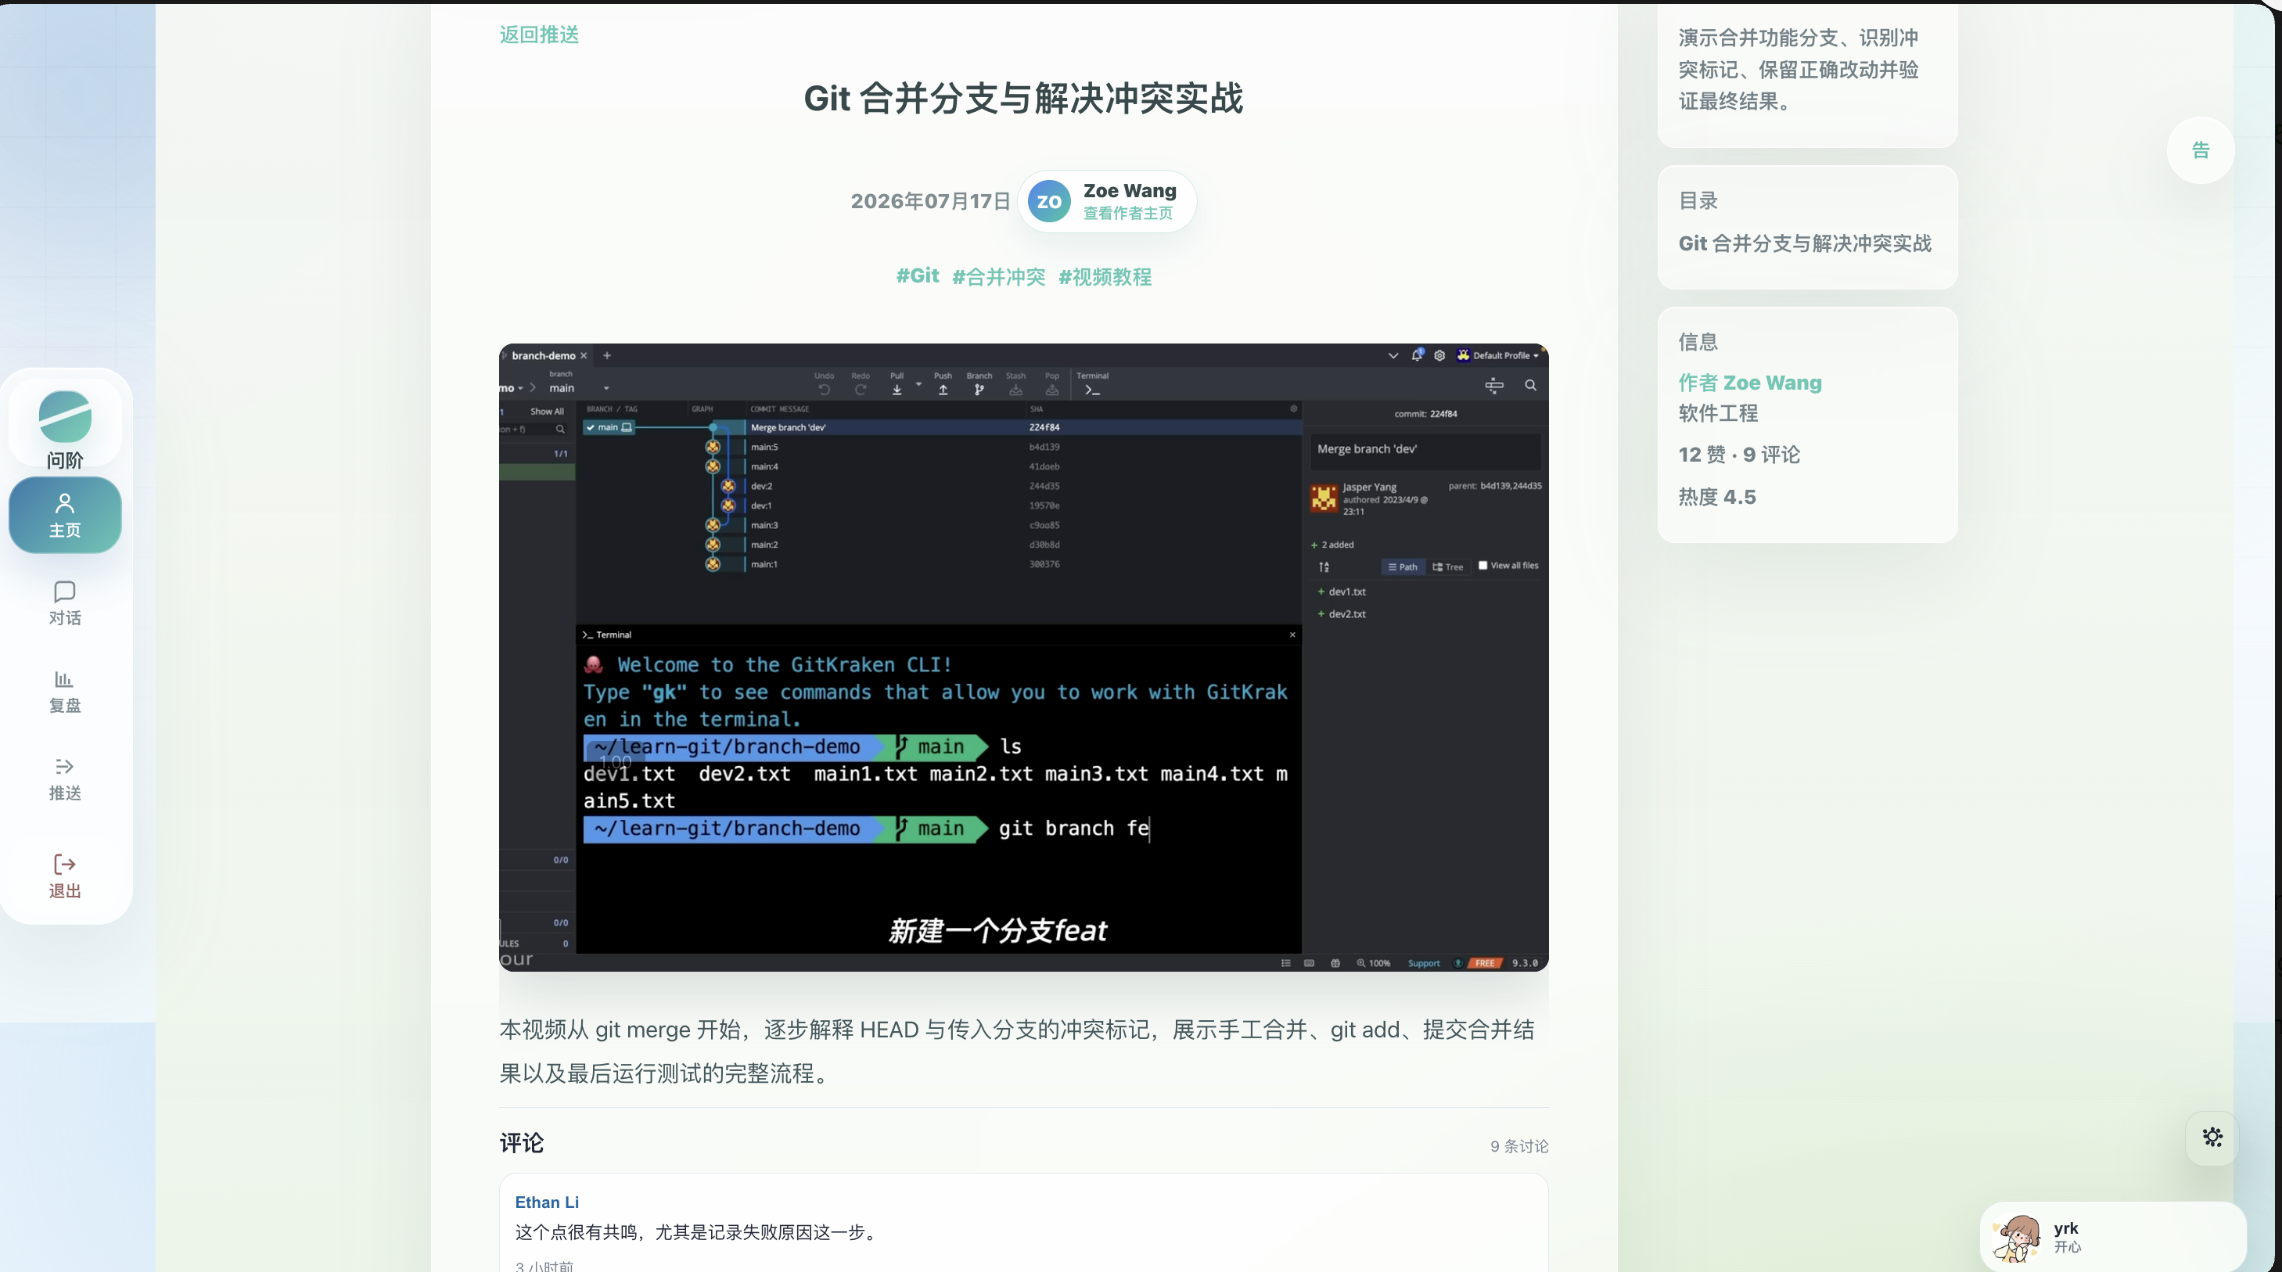
\includegraphics[width=\linewidth,height=1.95cm,keepaspectratio]{multimodal-video-detail.png}
\par\vspace{.3mm}
{\tiny\bfseries \textcolor{accentblue}{02}　视频可直接学习、评论与沉淀}
\par\vspace{.5mm}
\begin{minipage}[t]{.32\linewidth}

\includegraphics[width=\linewidth,height=1.08cm,keepaspectratio]{multimodal-voice.png}
\end{minipage}\hfill
\begin{minipage}[t]{.65\linewidth}
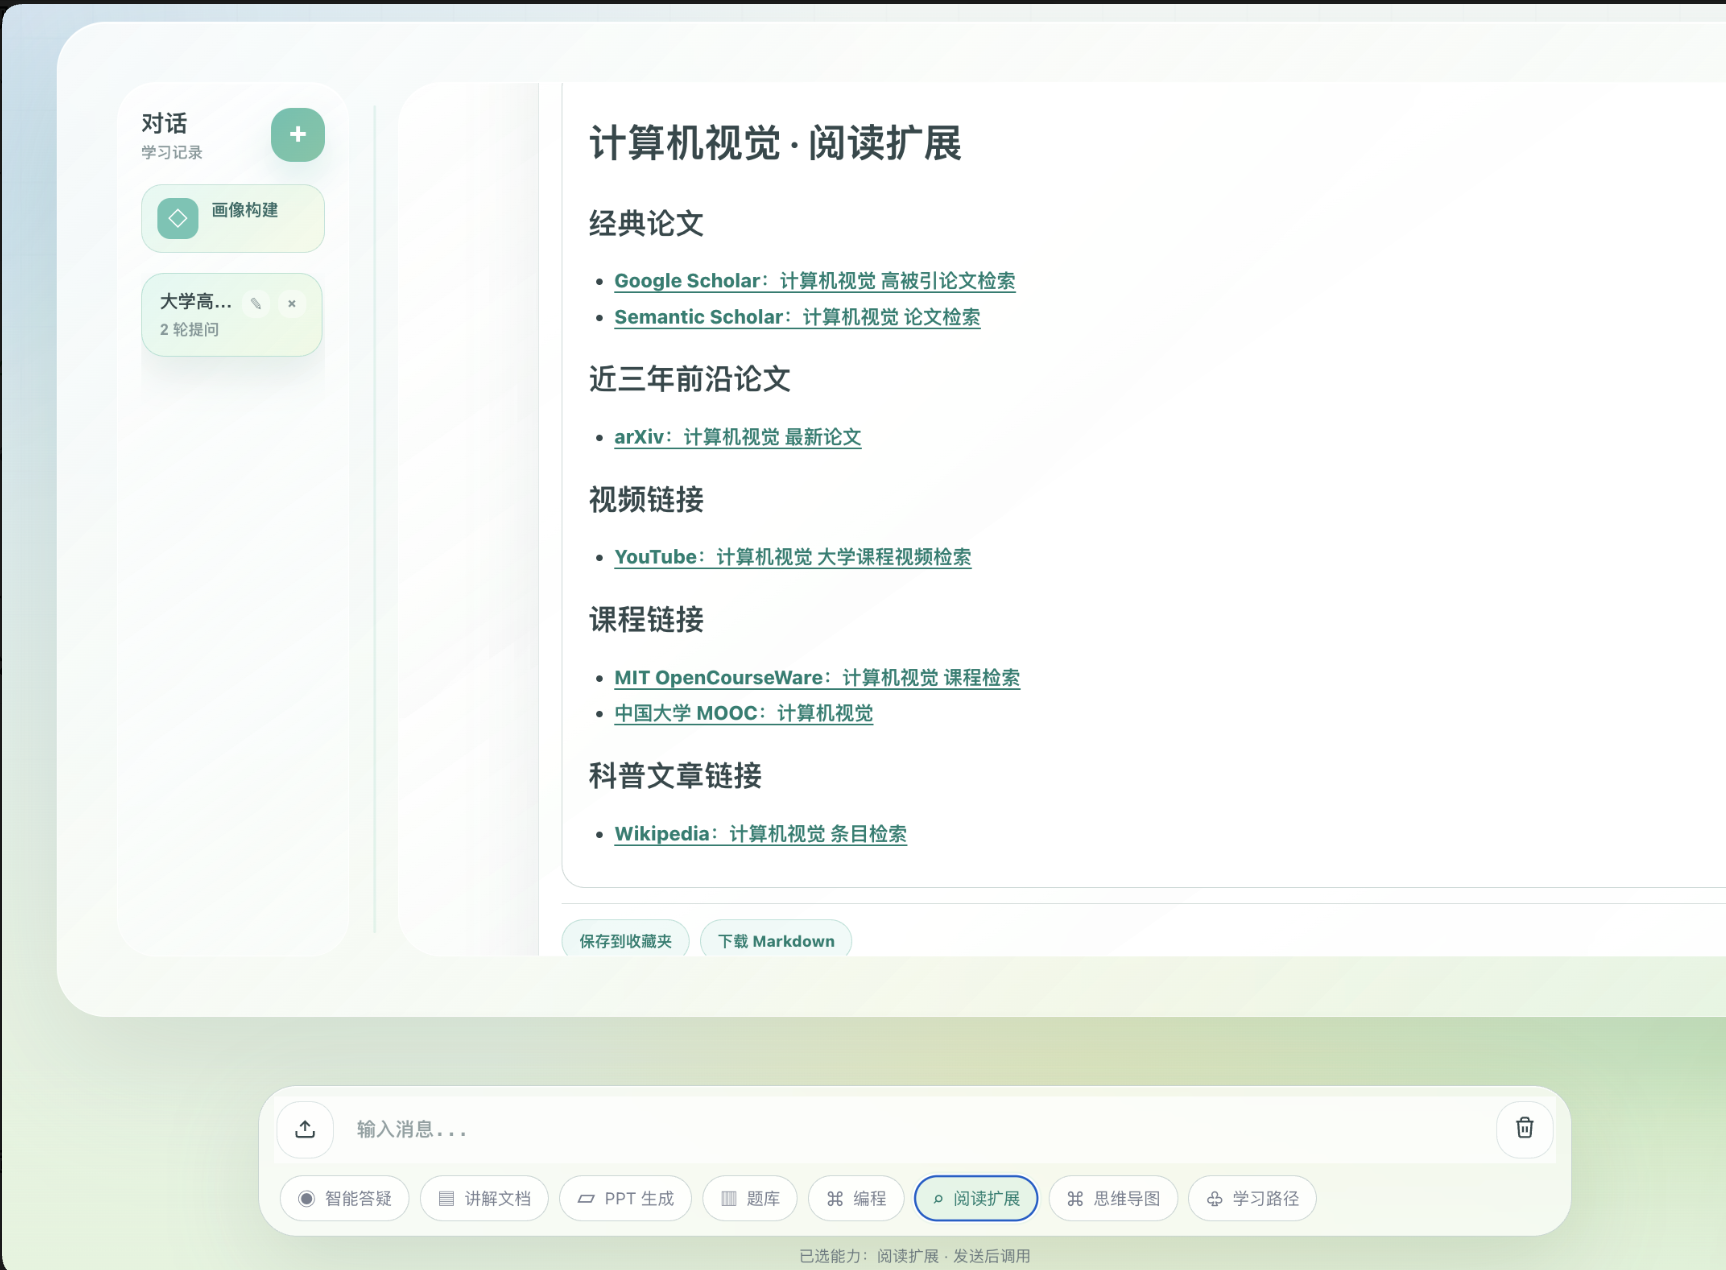
\includegraphics[width=\linewidth,height=1.08cm,keepaspectratio]{multimodal-reading.png}
\end{minipage}
\par\vspace{.3mm}
{\tiny\bfseries \textcolor{accentgreen}{03}　语音降低负担，延伸阅读衔接下一步}
\end{columns}
\vspace{1mm}
\begin{beamercolorbox}[wd=.94\textwidth,sep=1.5mm,center,rounded=true]{block body}
{\scriptsize\bfseries 根据学习阶段与掌握证据选择模态，把“读、看、听、练”编排成可执行路径。}
\end{beamercolorbox}
\end{frame}

\begin{frame}[shrink=15]{差异化价值：重构学习服务，而非叠加聊天入口}
\begin{tabular}{>{\bfseries}p{2.5cm}p{3.6cm}p{4.0cm}}
\toprule
比较维度 & 通用聊天式 AI & 问阶学习智能体\\
\midrule
学生理解 & 依赖当前对话，长期状态弱 & 8 维画像与需求轨迹持续更新\\
知识依据 & 主要依靠模型参数知识 & 完整课程 PDF、页码级 RAG、可信目录\\
资源生产 & 单次回答或单一文件 & 多角色 Agent 并行生成 7 类资源\\
内容形态 & 以文本回答为主，模态彼此分离 & 文本、图片、PDF、语音、视频、导图与 PPT 协同编排\\
学习行动 & 用户自行整理与安排 & 阶段、Todo、顺序理由和掌握证据\\
效果反馈 & 对话结束后链路中断 & 错题、正确率、使用与路径驱动再推荐\\
可信边界 & 生成与检索结果容易混淆 & 教材、可信检索、AI 扩展明确区分\\
\bottomrule
\end{tabular}
\vspace{4mm}
\begin{center}
{\large\bfseries 创新价值：从“内容生成”走向\textcolor{maincolor}{可验证、可执行、可进化}}
\end{center}
\end{frame}

\begin{frame}
\begin{center}
{\Huge\bfseries Thanks!}\par\vspace{5mm}

\includegraphics[width=.76\linewidth]{closing-slogan.png}\par\vspace{5mm}
{\Large\color{maincolor}\bfseries 让 AI 不只回答问题，更陪学生走完学习过程。}
\end{center}
\end{frame}

\end{document}
